
\documentclass[12pt]{article}
\usepackage[english]{babel}
\usepackage[utf8x]{inputenc}
\usepackage{amsmath}
\usepackage{graphicx}
\usepackage[colorinlistoftodos]{todonotes}
\usepackage[version=4]{mhchem}
\usepackage{mathtools}

\usepackage[margin=0.8in]{geometry}

\title{
   Combustion Processes in Thermochemical Propulsion\\
  \large Notes by Riccardo Canola}

\date{}

\begin{document}

\maketitle

\newpage

\tableofcontents

\newpage

\section{Phenomenological introduction to combustion processes}

Combustion is the development of chemical reactions of oxido-reduction, strongly exothermic and very fast, due to heat and catalyst products accumulation.
\begin{itemize}
    \item \textit{Diffusion flame}: the reactants diffuse into each other during the chemical reaction.
    \item \textit{Premixed flame}: the reactants are perfectly mixed before chemical reaction.
\end{itemize}

\begin{figure}[h!]
\centering
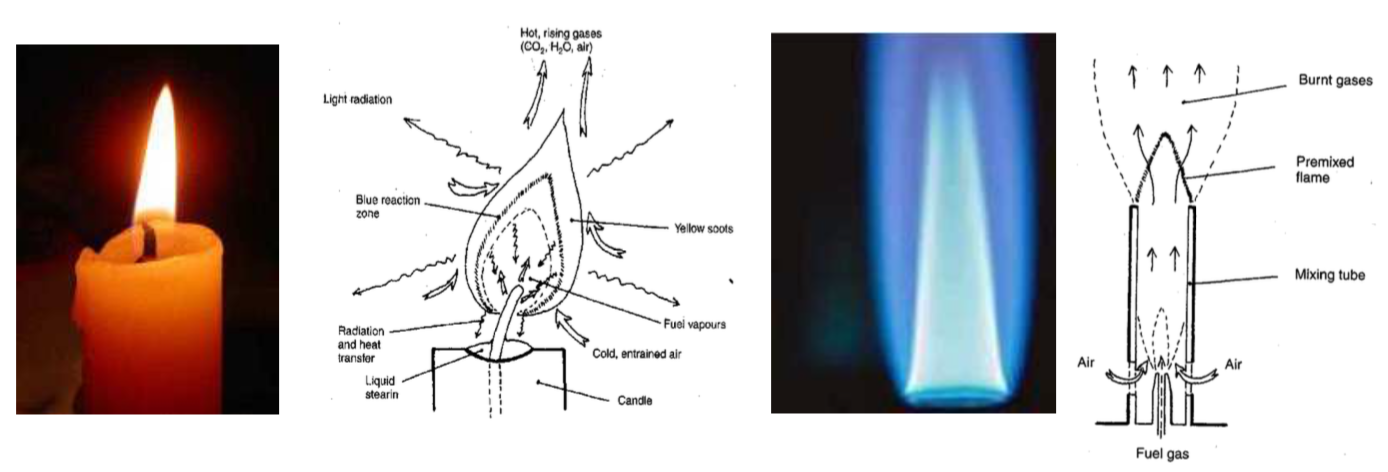
\includegraphics[width=0.8\textwidth]{figures/diffusion_premixed.png}
\end{figure}

\subsection{Industrial burners}

\begin{itemize}
    \item \textit{gas burners}: a swirler is responsible for high turbulence which increases flame speed propagation.
    \item \textit{liquid fuel burners}: the fuel is injected in form of spray. In order to anchor the flame, the air jet is introduced with a swirl motion, which causes a pressure drop and recirculation zone close to the central axis of the burner. The flame is longer and the soot is responsible for the higher radiation.
\end{itemize}

\subsection{Internal combustion engines}

\begin{itemize}
    \item \textit{Otto}: the combustion process in this kinf of engine which is spark-ignited, develop through a premixed flame with a laminar or turbulent flame propagation.
    \item  \textit{Diesel}: the combustion process develops through a diffusion flame and the flame speed propagation is turbulent.
\end{itemize}

\subsection{Ramjets}

Can be used above $Mach 2$. The gas velocity at the entrance of the combustion chamber is much faster than the flame propagation speed. The recirculation zone grants a permanence of the gas for several milliseconds. Temperature at turbine's blades has to be below a certain value.

\subsection{Rockets}

\begin{itemize}
    \item \textit{Liquid rocket}: they provide a good performance and permit re-ignition. The injector design is the most delicate aspect for the engine performance.
    \item \textit{Solid rocket}: fuel is a solid cylinder provided with a central perforation which forms the combustion chamber. The thrust is proportional to the combustion surface, therefore it is designed in a way that the combustion follows a rule ($r_{b}=ap^{n}$). The solid fuel (alluminum powder) contains the oxidizer and therefore the flame should be premixed. However, oxidizer decomposition products can react in diffusion flame. The interaction between premixed and diffusion flames is the most critical part of any modeling approach.
    
\begin{figure}[h!]
\centering
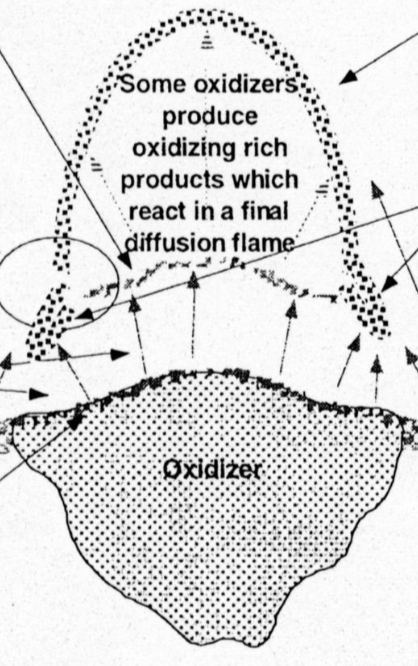
\includegraphics[width=0.3\textwidth]{figures/flame_solid.png}
\end{figure}
    
    \item \textit{Hybrid rocket}: fuel solid and oxidizer liquid. Oxidizer are introduced in form of spray. The flame develops inside the boundary layer ($r_{b}=aG_{ox}^{n}$).
    
\begin{figure}[h!]
\centering
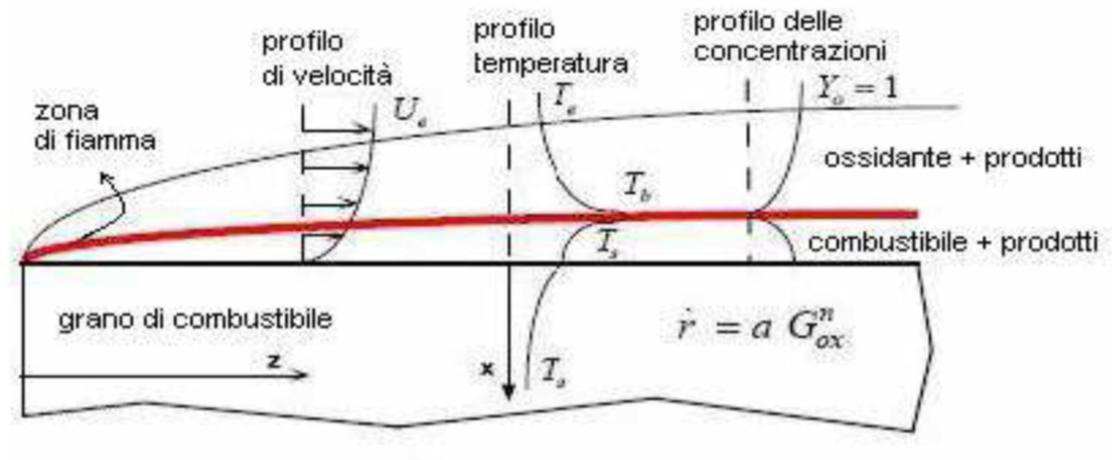
\includegraphics[width=0.8\textwidth]{figures/hybrid.png}
\end{figure}

\end{itemize}

\subsection{Flames}

Flame is a discontinuity surface separating reactants from combustion products. Its peculiar property is the capability of self-sustaining and propagation.

\begin{itemize}
    \item homogeneous and heterogeneous
    \item laminar and turbulent
    \item premixed and diffusion
    \item deflagration and detonation
\end{itemize}

\begin{figure}[h!]
\centering
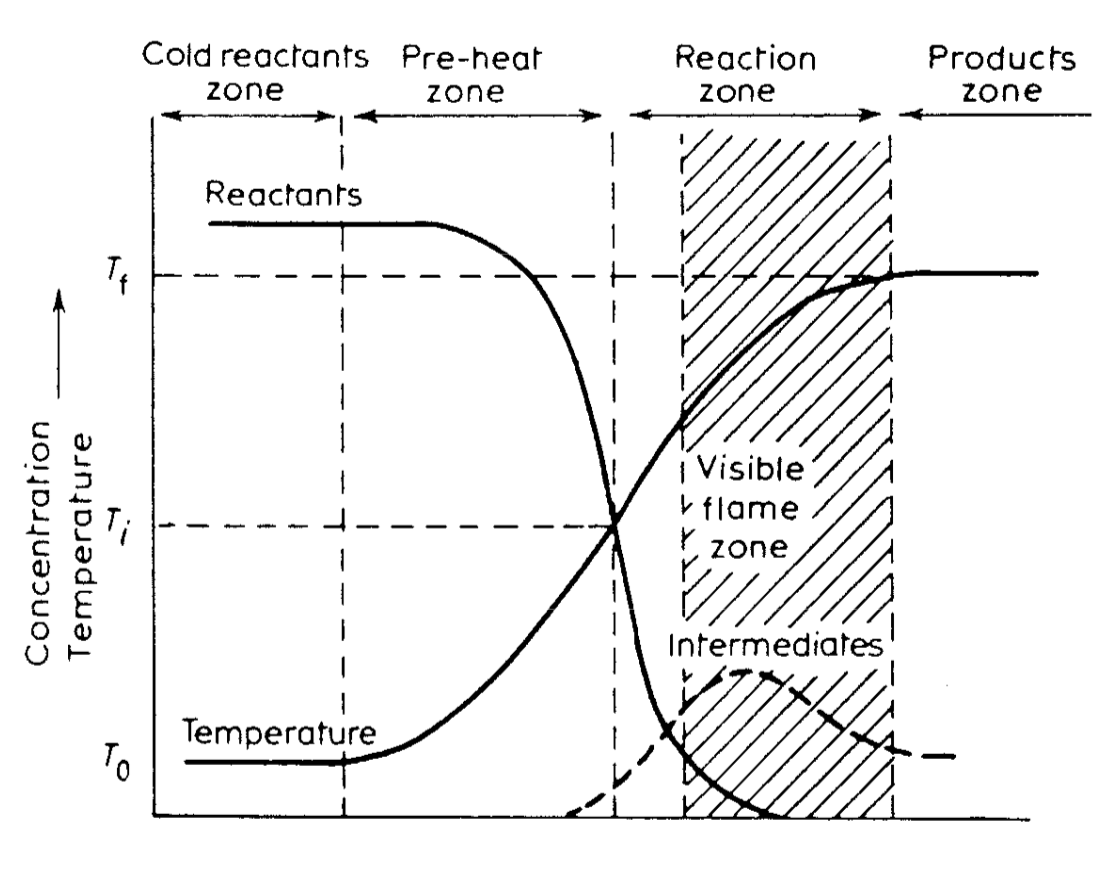
\includegraphics[width=0.5\textwidth]{figures/premixed_structure.png}
\caption{Premixed flame structure}
\end{figure}

\begin{figure}[h!]
\centering
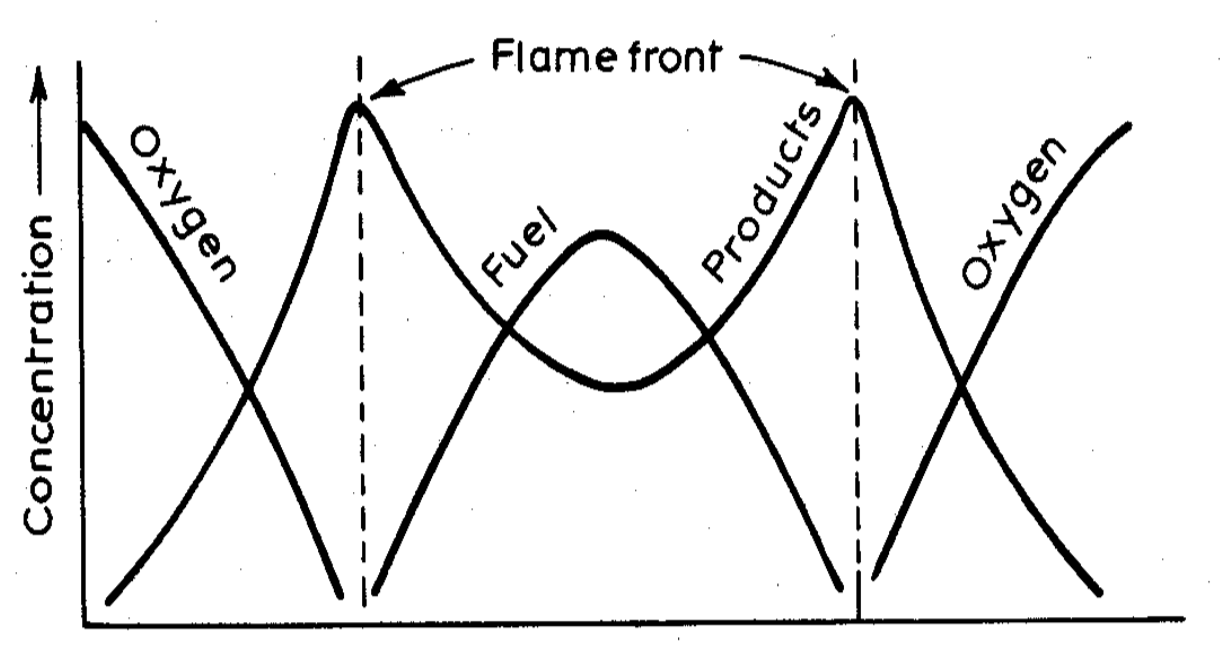
\includegraphics[width=0.5\textwidth]{figures/diffusion_structure.png}
\caption{Diffusion flame structure}
\end{figure}

\subsection{Flame propagation rate}

It is the speed relative to the fresh mixture. It is a constant for a specific mixture and it is proportional to the amount of mixture that in the time unit can be changed into combustion products.

\begin{itemize}
    \item methane/air: $0.4 m/s$
    \item methane/oxygen: $4.0 m/s$
    \item hydrogen/air: $1.8 m/s$
    \item hydrogen/oxygen: $10 m/s$
\end{itemize}

\subsection{Abiabatic flame temperature}

It is the temperature of combustion products in an adiabatic system. It depends on the fuel and oxidizer nature and on the mixture ratio.

\subsection{Mixture composition}

\begin{itemize}
    \item \textit{Mixture ratio} $\alpha$: amount of oxidizer, in mass or volume, linked to the fuel mass or volume unit.
    \item \textit{Equivalence ratio} $\phi$: mixture ratio normalized with respect to the stoichiometric ratio:
    \begin{equation}
        \phi = \frac{(Ox/F)}{(Ox/F)}_{stech}
    \end{equation}
    \item \textit{Air excess}: E.A.$=\phi-1$
\end{itemize}

\subsection{Inflammability limits}

Minimum volumetric concentration of fuel in the mixture (\textit{lower inflammability limit}) and maximum volumetric concentration of fuel in the mixture (\textit{upper inflammability limit}) in order to ignite the mixture. A mixture can be ignited only if the mixture ratio is within well defined limits.

\subsection{Reaction heat}

Energy released in the stoichiometric reaction of the fuel within molecular gaseous oxygen.

\subsection{Flash point}

Flash point of a liquid fuel is the lowest temperature at which, an amount of fuel vapour is produced which is able to be ignited by a suitable ignition device. The value decreases when pressure decreases and the oxygen content increases. The temperature of self-ignition is usually much higher than the temperature of the flash point. The two temperatures have a completely different physical meaning.

\newpage

\section{Fundamentals of chemical thermodynamics}

Thermochemistry provide a quantitative assessment of the energy released in a chemical reaction.
For a generic chemical equilibrium the mathematical formalism proposed by Penner is considered:

\begin{equation}
    \sum_{j=1}^{N} v_{i}^{'}M_{i} \rightarrow  \sum_{j=1}^{N} v_{i}^{''}M_{i}
\end{equation}

\begin{itemize}
    \item $M$ is the generic chemical substance
    \item $v^{'}$ are the stoichiometric coefficients relative to the reactants
    \item $v^{''}$ are the stoichiometric coefficients relative to the products
    \item $N$ is the total number of chemical components of the mixture

\end{itemize}

\subsection{Standard formation enthalpy $\Delta h_{f}^{0}$}

The standard enthalpy of formation $\Delta h_{f}^{0}$ of a substance at a given temperature is defined as the enthalpy of the substance obtained at the standard thermodynamic state.
\begin{itemize}
    \item The standard thermodynamic state of a given substance is the ideal gas or liquid or solid state that the substance assumes at the conditions of $p=1$ atm and temperature T.
\end{itemize}
The standard enthalpy of formation is a state property, therefore we are only interested in the initial and final state.

\subsection{Reaction enthalpy $\Delta h_{r}$}

The reaction enthalpy $(\Delta h_{r})_{T}$ at a given temperature T, is defined as the thermal energy released or absorbed during the reaction:
\begin{equation}
    \sum_{j=1}^{N} v_{i}^{'}M_{i} \rightarrow  \sum_{j=1}^{N} v_{i}^{''}M_{i} + \Delta h_{r}
\end{equation}
If the final temperature of the products is the same of the temperature of the reactants, the energy balance does not include contributions linked to the change of temperature:
\begin{equation}
    \Delta H_{r}=(\Delta h)_{T}^{0}= \sum_{products} v_{j}^{''}(\Delta h_{f}^{0})_{T} -\sum_{reactants} v_{j}^{'}(\Delta h_{f}^{0})_{T}
\end{equation}
This equation states that if the standard enthalpy of formation is known, the reaction enthalpy of any reaction can be evaluated.
\\
The energy released or absorbed has a definite value determined by the initial and final state:
\begin{itemize}
    \item for a reaction at constant pressure: $Q=\Delta H$
    \item for a reaction at constant volume: $Q=\Delta U$
\end{itemize}
the enthalpy totally involved, is given by:
\begin{equation}
    \Delta h_{r}= \sum_{products} v_{j}^{''}[\Delta (h_{f}^{0})_{T_{0}}+(h_{T_{2}}-h_{T_{0}})] -\sum_{reactants} v_{j}^{'}[\Delta (h_{f}^{0})_{T_{0}}+(h_{T_{1}}-h_{T_{0}})]
\end{equation}

\subsection{Reaction advancement}

The reaction advancement, defined as "$z$", is a molar concentration change. It is $z=0$ at the beginning of the reaction, and $z=1$ at the end. Consequently, the reaction enthalpy becomes $z\Delta u$ for a constant volume or $z\Delta h$ for a constant pressure.

\subsection{Fundamental thermochemical laws}

\begin{itemize}
    \item \textbf{Lavoisier and Laplace}: the energy associated to a chemical reaction in one direction is equal and opposite in sign, to the energy associated to the same reaction in the inverse direction.
    \item \textbf{Hess}: the energy associated to a chemical reaction at constant pressure or constant volume, is the same if the reaction is developed in one or more steps. It does not depend on the path, consequently, reactions can be treated as algebraic equations.
\end{itemize}

\subsection{Bond energies}

Bond energy is the energy required to break a bond between two atoms. Usually, this energy depends on the distance between atoms. It is necessary to consider the resonance in the molecule, which gives higher values of the standard formatioon enthalpy (it happens in the benzene $C_{6}H_{6}$).

\subsection{Adiabatic flame temperature}

The equation for the computation of the entalpy of reaction is:
\begin{equation}
    \Delta h_{r}= \sum_{products} v_{j}^{''}[\Delta (h_{f}^{0})_{T_{0}}+(h_{T_{2}}-h_{T_{0}})] -\sum_{reactants} v_{j}^{'}[\Delta (h_{f}^{0})_{T_{0}}+(h_{T_{1}}-h_{T_{0}})]
\end{equation}
if the heat released is used to heat the products, the products temperature $T_{2}$ is defined as \textit{adiabatic flame temperature}, therefore $(\Delta h_{r})=0$ and the equation becomes:
\begin{equation}
    \sum_{products} v_{j}^{''}[\Delta (h_{f}^{0})_{T_{0}}+(h_{T_{2}}-h_{T_{0}})] =\sum_{reactants} v_{j}^{'}[\Delta (h_{f}^{0})_{T_{0}}+(h_{T_{1}}-h_{T_{0}})]
\end{equation}
if the products are known, it is possible to obtain the flame temperature.
\\
The heat released to the combustion products under adiabatic conditions is:
\begin{equation}
    -\Delta H_{r} = N_{tot}C_{P}\Delta T_{adiabatic}
\end{equation}
\begin{equation}
    \Delta T_{adiabatic} = \frac{\Delta H_{r}}{C_{P}N_{tot}}
\end{equation}
 For high temperature \textit{dissociation reactions} (strongly endothermic) develop. They produce other species ($CO, H_{2},...$), decreasing the global exothermicity of the reaction and the adiabatic flame temperature.
\begin{figure}[h!]
\centering
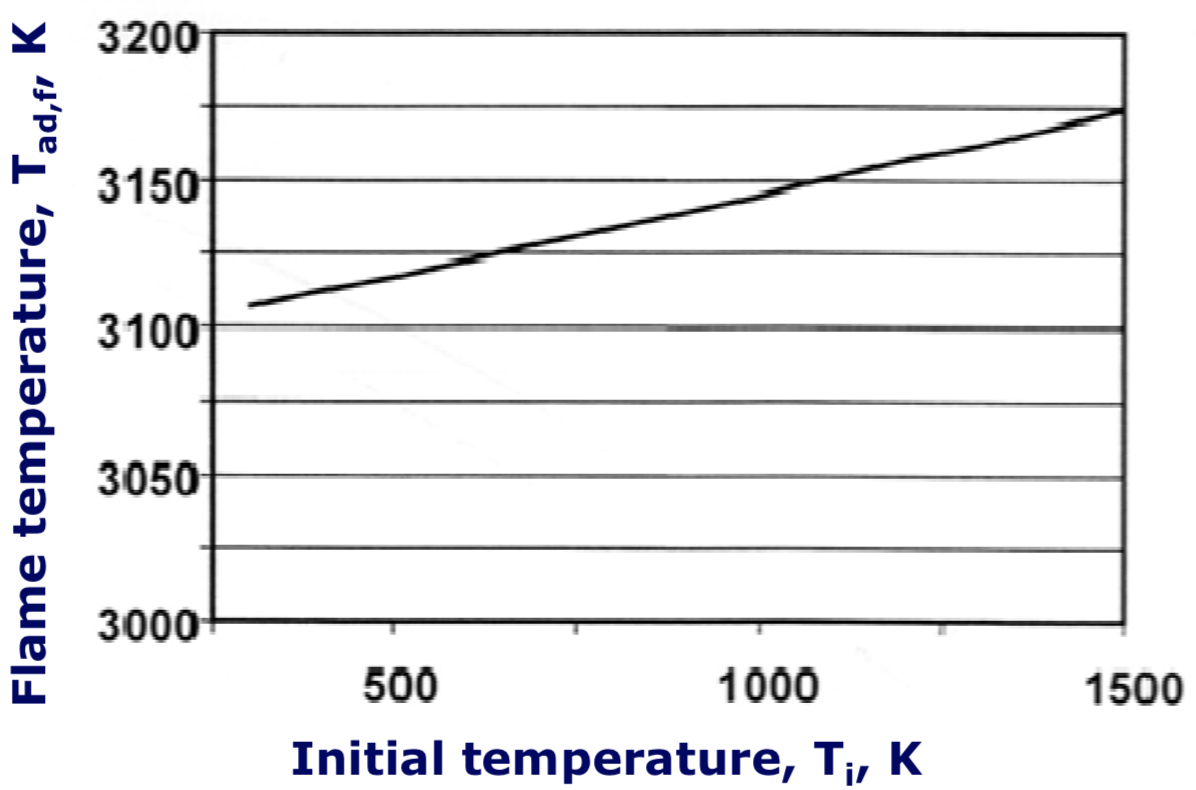
\includegraphics[width=0.5\textwidth]{figures/dissociation.png}
\end{figure}
Trend of the adiabatic flame temperature, significant increases of $T_{i}$ cause modesr increases of $T_{ad}$ due to dissociation reactions.

\subsection{Equilibrium ($K_{p}$)}

Chemical equilibrium is one of the most important concepts in thermochemical propulsion. It assumes that at the exit from the combustion chamber, chemical phenomena behave as quasi-steady (much faster) with respect to the fluid dynamic phenomena:
\begin{equation}
    \frac{t_{ch}^{*}}{t_{fl}^{*}} << 1
\end{equation}
A system is in a stable equilibrium when its state can be changed reversibly by an infinitesimmal amount. Such system obeys to the relationship:
\begin{equation}
    TdS=de+pdV=dh-Vdp
\end{equation}
combustion processes are characterized by constant pressure and temperature, therefore the condition can be rewritten as:
\begin{equation}
    d(e+pV-TS)_{p,T}=d(h-TS)_{p,T}=0
\end{equation}
where the \textit{Gibbs free energy}, is:
\begin{equation}
    F=(e+pV-TS)=h-TS
\end{equation}
Thus, the stable equilibrium condition of any chemical system working at constant temperature and pressure, is:
\begin{equation}
    (dF)_{p,T}=0
\end{equation}
It is possible to show that the criterium of stable equilibrium to small perturbations leads to:
\begin{equation}
    \Delta F^{0}(T)=-RTlnK_{p} = \sum_{j=1}^{N}(v_{j}^{''}-v_{j}^{'})F_{j}^{0}
\end{equation}
\begin{equation}
    K_{p}(T)= \frac{\prod_{j=1}^{N}(p_{j})^{v_{j}^{''}}}{\prod_{j=1}^{N}(p_{j})^{v_{j}^{'}}}
\end{equation}
$K_{p}$ is the \textit{equilibrium constant} and $p_{j}$ are the partial pressure of the mixture.

\subsection{The physical meaning of $K_{p}$}

The more negative $\Delta F^{0}$ is, the larger is $K_{p}$. This means that the reaction is more spontaneous. When the free energy of the reactants and products is the same, the reaction has no tendency to proceed in either direction.
The practical importance of $K_{p}$ is that it is independent on total pressure and can be a unique function of the temperature.
\begin{equation}
    \Delta F^{0}(T)=-RTlnK_{p}
\end{equation}
Since the variation $\Delta F^{0}$ depends only on temperature also the second member depends only on temperature.
Consequently, for a given mixture it is possible to tabulate $K_{p}(T)$. This is an extremely interesting result for propulsion applications since the free energy change at the standard pressure $p=1 atm$ determines the equilibrium conditions at all other pressure.
\begin{equation}
    \Delta F_{p,T}=0
\end{equation}
is the equilibrium condition (not $\Delta F^{0}$!)

\subsection{Equilibrium constants}

\begin{itemize}
    \item $K_{p}=\prod_{j=1}^{N}(p_{j})^{{v_{j}^{''}}-{v_{j}^{'}}} \rightarrow$ partial pressure
    \item $K_{n}=\prod_{j=1}^{N}(n_{j})^{{v_{j}^{''}}-{v_{j}^{'}}} \rightarrow$ number of partial moles
    \item $K_{X}=\prod_{j=1}^{N}(X_{j})^{{v_{j}^{''}}-{v_{j}^{'}}} \rightarrow$ partial molar function
    \item $K_{c}=\prod_{j=1}^{N}(M_{j})^{{v_{j}^{''}}-{v_{j}^{'}}} \rightarrow$ partial molar concentration
    \item $K_{Y}=\prod_{j=1}^{N}(Y_{j})^{{v_{j}^{''}}-{v_{j}^{'}}} \rightarrow$ partial mass fraction
\end{itemize} 
but only $K_{p}$ and $K_{c}$ are functions of just one variable and don't depend on pressure. Propulsion applications preferably uses $K_{p}$.

\subsection{Mixture composition and flame temperature}

The problem of thermochemical equilibrium in combustion chambers requires to know simultaneously temperature and composition of the mixture (mass and energy conservation equations).\\
We can decouple the problem.

\subsubsection{Flame temperature}

We suppose the combustion chamber as an open thermodynamic system, where chemical reactions occur at constant pressure And we suppose known the composition of the reactive mixture before and after the reactions.

\begin{equation}
    \sum_{j=1}^{N}n_{j}^{'}\{(\Delta h_{f}^{0})_{T_{ref}}+[\Delta h^{0}]_{T_{ref}}^{T_{j}}\}_{j} \rightarrow
    combustor
    \rightarrow
    \sum_{j=1}^{N}n_{j}^{''}\{(\Delta h_{f}^{0})_{T_{ref}}+[\Delta h^{0}]_{T_{ref}}^{T_{c}}\}_{j}
\end{equation}

$T_{j}$ is the temperature of injection of $n_{j}$ moles of reactants in the combustion chamber, and $T_{c}$ is the common temperature of exit from the combustion chamber of the $n_{j}$ moles of products.
$T_{ref}$ is the reference table of the available tables.\\
The energy conservation requires:

\begin{equation}
    \sum_{j=1}^{N}n_{j}^{'}[(\Delta h_{f}^{0})_{T_{ref}}+(h_{T_{j}}^{0}-h_{T_{ref}}^{0})]_{j}
    =
    \sum_{j=1}^{N}n_{j}^{''}[(\Delta h_{f}^{0})_{T_{ref}}+(h_{T_{c}}^{0}-h_{T_{ref}}^{0})]_{j}+\Delta h_{ext}
\end{equation}

where $h_{T}^{0}-h_{T_{ref}}^{0} = \int_{T_{ref}}^{T} Cp_{j}(T)dT$ are tabulated values of the molar thermal enthalpy.\\
The temperature $T_{C}$ resulting from the conservation energy equation is called \textit{flame temperature}. It increases if enthalpy lost to the environment decreases. If $\Delta h_{ext}=0$, the adiabatic flame temperature is the maximum admissible temperature in the combustion chamber.

\subsubsection{Available and absorbed enthalpy}

\begin{equation}
    \Delta h_{available}^{0} = \left\{
    \sum_{j=1}^{N}n_{j}^{'}[(\Delta h_{f}^{0})_{T_{ref}}+(h_{T_{j}}^{0}-h_{T_{ref}}^{0})]_{j}
    -
    \sum_{j=1}^{N}n_{j}^{''}[(\Delta h_{f}^{0})_{T_{ref}}]_{j}\right\} - \Delta h_{ext}
\end{equation}

is the enthalpy available due to chemical reactions, while:

\begin{equation}
    \Delta h_{absorbed}^{0} = \sum_{j=1}^{N}n_{j}^{''}(h_{T_{c}}^{0}-h_{T_{ref}}^{0})_{j}
\end{equation}

is the enthalpy absorbed to warm up the combustion products.

\begin{figure}[h!]
\centering
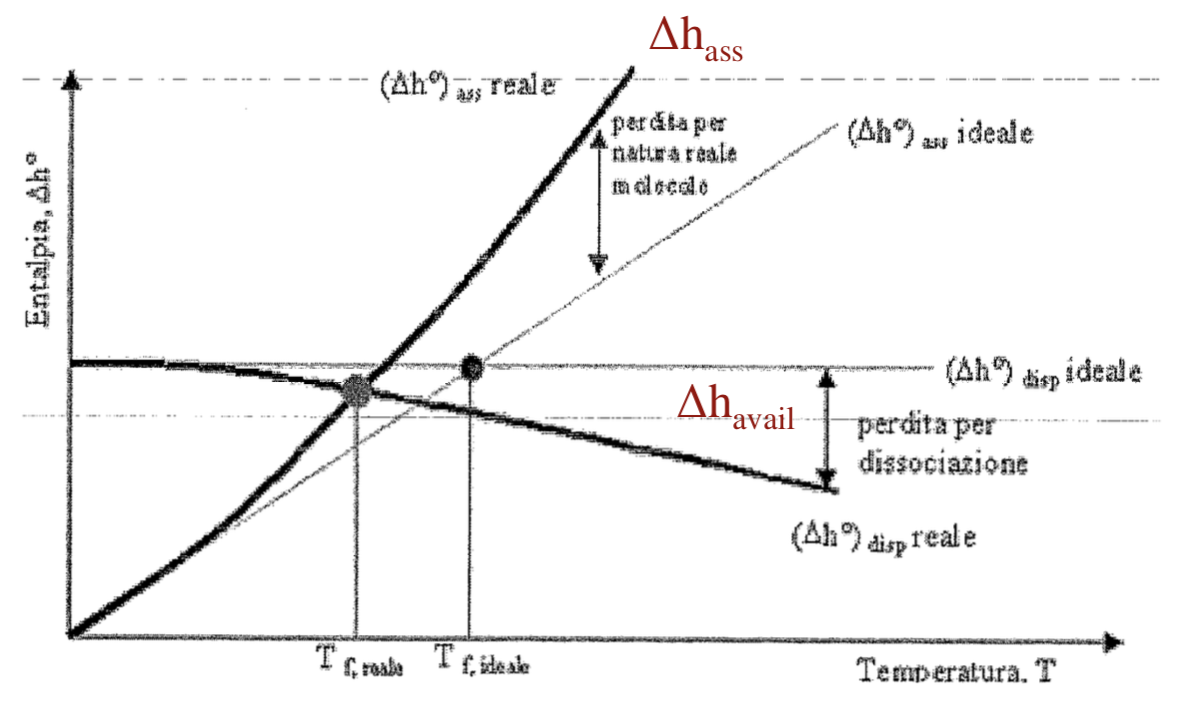
\includegraphics[width=0.6\textwidth]{figures/availablevsabsorbed.png}
\end{figure}

Increasing combustion temperature implies a fall in the available enthalpy due to molecular dissociation and the simultaneous growth of the absorbed enthalpy.\\
These phenomena, show a limit of operations for all thermal propulsion system which is approximately at $5000 K$.

\subsubsection{Mixture composition}

In this case it is knownn the working pressure $p_{c}$, $T_{j}$, $T_{c}$.

\begin{equation}
    n_{j}^{'} \rightarrow n_{j}^{''}?
\end{equation}

\newpage

\section{Fundamentals of chemical kinetics in combustion processes}

\begin{itemize}
    \item Chemical thermodynamics involves systems containing a high number of chemical species. The considered chemical quantity is the \textit{mole}.
    \item Chemical kinetics focuses on systems in which singular species are involved. The considered chemical quantity is the \textit{molecule}.
\end{itemize}

The study of the thermodynamic aspects of combustion only require the global reaction. However, when mechanisms involved in the reaction process are many, they cannot occur in one step of reaction. The singular step is named \textit{elementary reaction} and the set of elementary reactions is the so called \textit{reaction mechanism}.\\
In this section we study the rate of change at which elementary reactions develop, and the governing laws of the reaction rate.\\
Then the important concept of \textit{chain of reactions} is introduced.\\
Chemical reactions can be divided, looking at the reaction rate, into:
\begin{itemize}
    \item reactions of \textit{explosive nature}
    \item reactions of non-explosive nature
\end{itemize}
The explosive nature (high reaction rate) characterizes the combustion systems, but reactions non-explosive are also important (production of pollutants).

\subsection{Chemical reaction rate}

The reaction rate \textbf{$\dot{\omega}$} [$\frac{mole}{cm^{3}s}$] depends on:
\begin{itemize}
    \item concentration of reactants
    \item temperature (T)
    \item pressure (p)
    \item presence of catalysts or reaction inhibitors
    \item radiant effects
\end{itemize}
and can be expresses as the concentration rate decresase of one reactant, or concentration rate increase of a produced species.\\
Consider the elementary reaction in a closed system:
\begin{equation}
    aA+bB+... \rightarrow cC+dD+...
\end{equation}
now, let's define \textit{z} the reaction development:
\begin{equation}
    -\frac{dn_{A}}{a}dt =
    -\frac{dn_{B}}{b}dt =
    +\frac{dn_{C}}{c}dt =
    \frac{dz}{dt}
\end{equation}
and the reaction rate can be defines as:
\begin{equation}
    \dot{\omega} = \frac{dz}{dt}
\end{equation}
and does not depend on the chemical species considered.

\subsection{Law of mass action}

The chemical reaction is given by:
\begin{equation}
    \dot{\omega} = k \prod_{i=1}^{N}[M_{i}]^{v_{i}}
\end{equation}
where $K$ is the \textit{rate constant} which depend only on temperature T given by Arrhenius Law.

\subsection{Molecular collision theory}

Essential requirement for the occuring of an elementary reaction is that species come in contact. The reaction rate cannot be higher than the \textit{collision frequency} between A and B, named \textbf{$Z_{AB}$} which for gasses is given by the gas kinetic theory.\\
Real rate is $10^{10}$ times lower of the collision frequency $Z_{AB}$. Also, collision have to be considered effective only if their energy is higher than a \textit{treshold value} \textit{$E_{a}$}.

\subsection{The activated complex theory}

\begin{equation}
    X+YZ \rightarrow XY+Z
\end{equation}
$d_{YZ}$ is the distance between Y and Z and $d_{XY}$ is the distance between X and Y. The curves of the picture are curves at equal potential energy. Stability is given by two valleys. For the initial system point a and for the final system point b.
The transition from the intial system to the final system requires the moving from the first valley to the second, following the path which is the most efficient from the energetic point of view, crossing c (\textit{punto di sella}). The crossing of the point c can occur if the system receives a suitable amount of energy (molecular vibrations) that is given by an exponential term ($E_{a}/RT$) which explains the concepts of efficient collision which leads to the \textit{activated complex}.

\begin{figure}[h!]
\centering
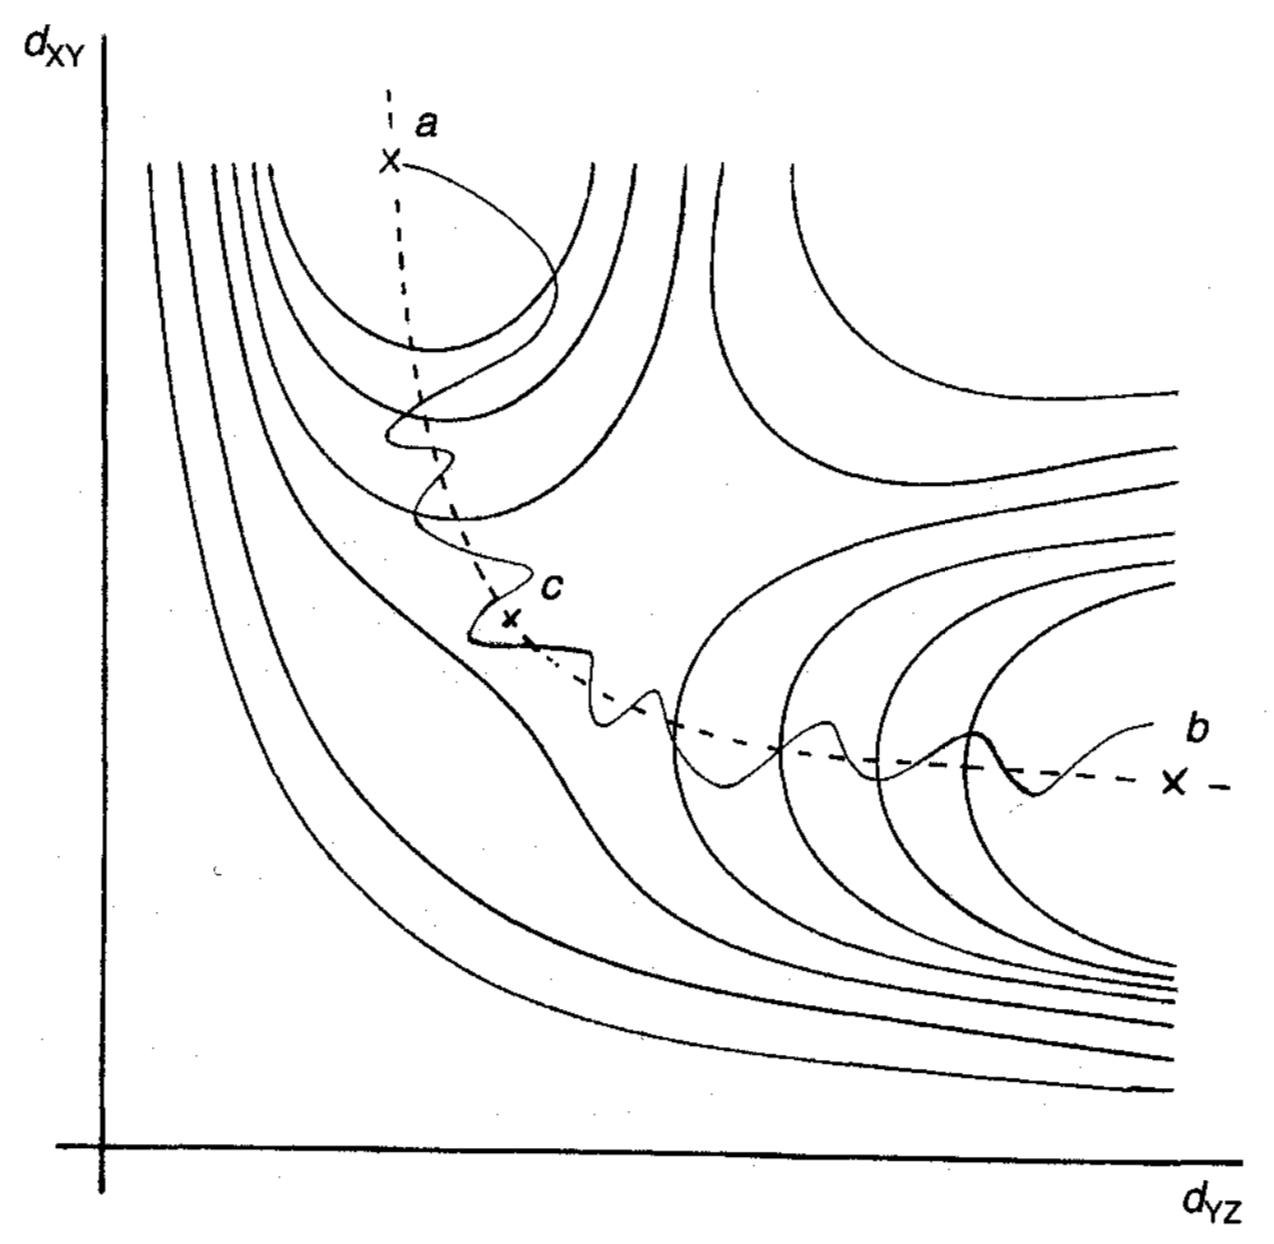
\includegraphics[width=0.35\textwidth]{figures/pointc.png}
\end{figure}



\subsection{Arrhenius law}

\begin{figure}[!htb]
    \centering
    \begin{minipage}{.5\textwidth}
        \centering
        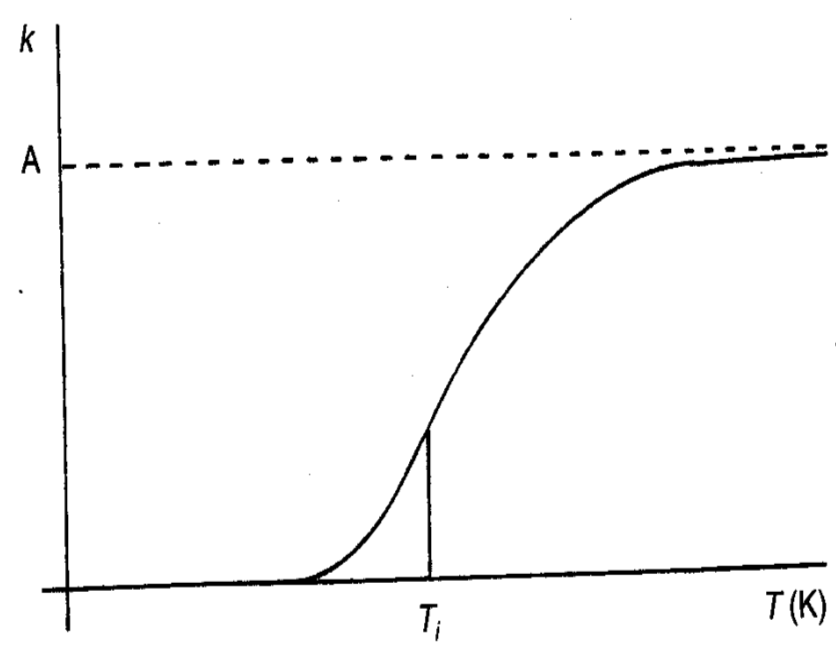
\includegraphics[width=0.8\linewidth, height=0.15\textheight]{figures/arr1.png}
    \end{minipage}%
    \begin{minipage}{0.5\textwidth}
        \centering
        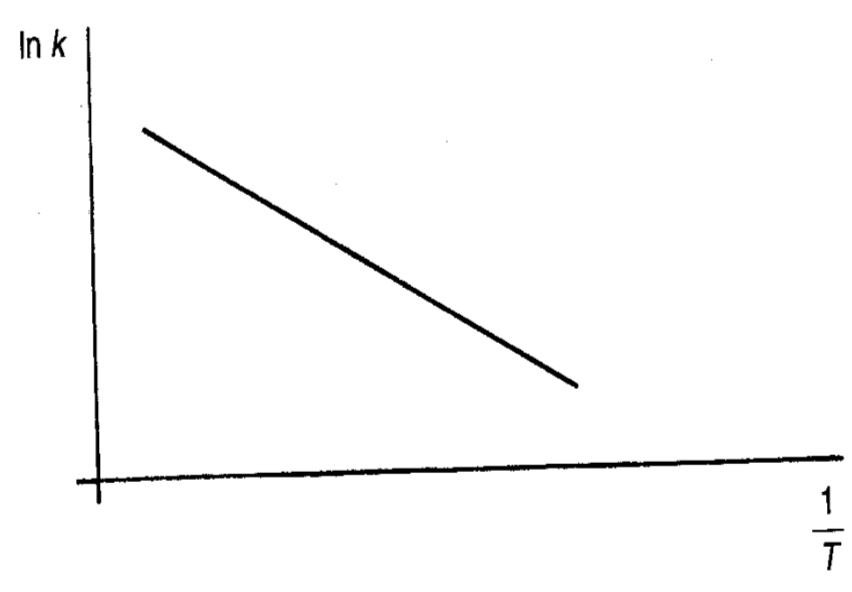
\includegraphics[width=0.8\linewidth, height=0.15\textheight]{figures/arr2.png}
    \end{minipage}
\end{figure}

Trend of the rate constant vs temperature according to the Arrhenius Law ($lnK=g(1/T)$). $K$ tends to the frequency factor when the temperature becomes very high. Reactions kinetics are investigated significantly below this limit.

\begin{equation}
    K=BT^{a}e^{-E_{a}/RT}
\end{equation}
where $BT^{a}$ is the collision frequency and $e^{-E_{a}/RT}$ is the Boltzmann factor (the fraction of collisions which have an energy larger than the activation energy $E_{a}$).\\
Thus, for a second order reaction:
\begin{equation}
    B+C \rightarrow products
\end{equation}
the reaction is given by:
\begin{equation}
    \frac{d[B]}{dt} = - K[B][C] = -A[B][C]e^{-E_{a}/RT}
\end{equation}
where $A=BT^{a}$.
Given a chemical reaction, the specific reaction rate does not depend on concentrations $[M]_{i}$, it depends only on temperature.

\subsection{Activation energy}

A collision leads to the formation of a transient chemical species, an aggregate which is defined activated complex $X^{+}$. The energy between two atoms of a diatomic molecul ($A_{2}$) depends on the distance between the two atoms. When an atom B becomes closer to the molecul, the distance between the atoms A and A changes. The collision of B with $A_{2}$ leads to the formation of the activated complex $BA_{2}^{+}$ , which has a much higher reactivity than that of neutral atoms.\\
The reaction follows the reaction path with the lowest energy among all possible paths.

\begin{itemize}
    \item the activation energy for direct and indirect reactions is not the same
    \item the direct and reverse reactions have different rate constant
    \item $E_{a}$ is the required energy in order to develop the reaction, it is the energy to bring reactants over the energy treshold needed
\end{itemize}

\subsection{Reaction order}

The net rate of production of a chemical species is given by:
\begin{equation}
    \frac{d[M]_{i}}{dt} = (v_{i}^{''}-v_{i}^{'})\dot{\omega}=(v_{i}^{''}-v_{i}^{'})K_{f}\prod_{i=1}^{N}[M]_{i}^{v_{i}^{'}}
\end{equation}
The reaction process is of order $v_{i}^{'}$ respect to $M_{i}$, the \textit{global reaction order m} is given by:
\begin{equation}
    m = \sum_{i=1}^{N}v_{i}^{'}
\end{equation}
in other words, the sum of the exponents of the reactants concentration terms.

\subsection{One-step chemical reactions}

\subsubsection{First order reactions}

\begin{itemize}
    \item Decomposition of the molecule: $A_{2}\xrightarrow{k_{f}} 2A$
    \begin{equation}
        \frac{d[A]}{dt}=2K_{f}[A_{2}]
    \end{equation}
    \item Dissociation of the molecule:
    $AB\xrightarrow{k_{f}} A+B$
    \begin{equation}
        \frac{d[AB]}{dt}=-K_{f}[AB]
    \end{equation}
    \item Bimolecular reaction:
    $A+C\xrightarrow{k_{f}} D$ \\where $[C]>[A]$
    \begin{equation}
        \frac{d[A]}{dt}=-\frac{d[D]}{dt}=-K_{f}[A][C]=k'[A]
    \end{equation}
    $k'$ is a new specific rate constant, defined considering that $[C]=constant$.
\end{itemize}
All monomolecular reactions are of order 1, but not all the first order reactions are monomolecular.

\subsubsection{Second order reactions}

Often chemical reactions follow second order reactions. In more complex reaction, the second order means that the slow step, which is responsible for the reaction rate, is bimolecular.
\begin{equation}
 A+B\xrightarrow{k_{f}} AB   
\end{equation}
    \begin{equation}
        \frac{d[AB]}{dt}=K_{f}[A][B]=-\frac{d[A]}{dt}=-\frac{d[B]}{dt}
    \end{equation}
\begin{equation}
   2A\xrightarrow{k_{f}} C+D 
\end{equation}
    \begin{equation}
        2\frac{d[C]}{dt}=2\frac{d[D]}{dt}=2K_{f}[A]^{2}=-\frac{d[A]}{dt}
    \end{equation}

\subsubsection{Third order reactions}
\begin{itemize}
    \item Trimolecular reaction:
    \begin{equation}
    2NO+O_{2}\xrightarrow{k_{f}} 2NO_{2}
    \end{equation}
    \item Involvement of a third body:
    \begin{equation}
    M+2A_{2}\xrightarrow{k_{f}} A_{2}+M^{*}
    \end{equation}
    \begin{equation}
        \frac{d[A_{2}]}{dt}=k_{f}[M][A]^{2}=-\frac{1}{2}\frac{d[A]}{dt}
    \end{equation}
    \begin{equation}
        \frac{d[A]}{dt}=-2k_{f}[M][A]^{2}
    \end{equation}
\end{itemize}
If $[M]=const,  \frac{d[A]}{dt}=-k'[A]^{2}$\\ in this case the reaction order is reduced from 3 to 2.

\subsection{Consecutive Reactions}

\begin{equation}
    A+B\xrightarrow{k_{2}}AB\xrightarrow{k_{2}}C+D
\end{equation}
\begin{equation}
        \frac{d[AB]}{dt}=k_{1}[A][B]=-\frac{d[A]}{dt}=-\frac{d[B]}{dt}
\end{equation}
\begin{equation}
        \frac{d[AB]}{dt}=k_{2}[AB]=-\frac{d[C]}{dt}=-\frac{d[D]}{dt}
\end{equation}
\begin{equation}
        \frac{d[AB]}{dt}=k_{1}[A][B]-k_{2}[AB]
\end{equation}

With the development of the reaction, the concentrations of A and B decrease, and the concentrations of C and D increase.

\subsection{Competitive reactions}

\begin{equation}
    A+B\xrightarrow{k_{1}}AB
\end{equation}
\begin{equation}
    A+B\xrightarrow{k_{2}}E+F
\end{equation}

\begin{itemize}
    \item $1^{st}$ reaction:
    \begin{equation}
        \frac{d[A]}{dt}=-k_{1}[A][B]
    \end{equation}
     \item $2^{nd}$ reaction:
    \begin{equation}
        \frac{d[A]}{dt}=-k_{2}[A][B]
    \end{equation}
    \begin{equation}
        \frac{d[A]}{dt}=-(k_(1)+k_{2})[A][B]
    \end{equation}
\end{itemize}
The specific rate constant can depend on temperature. The extrapolation of the rate law, obtained in a certain temperature interval, could lead to a mistake if extrapolated to a higher temperature interval.

\subsection{Opposite reactions}

TODO

\newpage

\section{Laminar premixed and diffusion flames}

A flame, which depends on the interplay of chemical and physical processes, is caused by the self-propagating of exothermic reaction. Two properties can be defined and measured: the \textit{burning rate or flame propagation rate ($S_{i}$)} and the \textit{adiabatic flame temperture ($T_{f,ad}$)}. \\
Burning rate increases at reduced pressure and at elevated temperatures. The mixture ratio at stoichiometric conditions lead to a maximum value.\\
The flame will be held at a fixed position (stationarity) since the gas flow rate is equal in magnitude, but opposite in sign, to the burning rate.\\
The goal is to predict the value of the burning rate from knowledge of the physical and chemical properties.

\subsubsection{The Mallard - Le Chatelier Model (P)}

It is assumed:
\begin{itemize}
    \item $(T_{f}-T{i}/\delta_{r})$ is the temperature gradient where $\delta_{r}$ is the reaction zone thickness
    \item $\lambda(T_{f}-T{i}/\delta_{r})$ is the \textit{heat flux} where $\lambda$ is the thermal conductivity
    \item the heat flux must be equal to the increase of enthalpy $\dot{m}C_{p}(T_{i}-T{0})$
    \item $\dot{m}=S_{L}\rho$ is the mass flow for a one-dimensional system, where \textbf{$S_{L}$} is the \textit{flow velocity}.
\end{itemize}
Therefore:
\begin{equation}
    S_{L} = \bigg[\frac{\lambda(T_{f}-T{i})\dot{\omega}}{\rho C_{p}(T_{i}-T{0}}\bigg]^{\frac{1}{2}}
\end{equation}
As $\frac{\lambda}{\rho C_{p}} = \alpha$ is the \textit{thermal diffusity}, the approach lads to the important conclusion that:
\begin{equation}
    S_{L}\sim[\alpha \dot{\omega}]^{\frac{1}{2}}
\end{equation}

which is not an accurate calculation of the burning rate (flame propagation rate), but enables to take into account parameters to be then predicted with some precision.

\subsubsection{Propagation by active species (P)}

The Mallard - Le Chatelier model assumes that the flame propagation is due entirely to heat conduction. A new model propose that the diffusion of active species ahead of the flame could provide an other explanation (\textit{thermal vs diffusional theories}).\\
A theory based purely on diffusion assumes isothermal propagation and that the equilibrium is attained at the end of the reaction zone. Then, the \textit{active centers} diffuse upstream into the reaction zone where their concentrations are in excess of equilibrium values for the given temperature.\\
A concentration profile can be found by solving the diffusion equation and the following burning rate is obtained:

\begin{equation}
    S_{L}^{2} =\frac{\sum_{j}K_{j}[F]X_{j}D_{j0}}{X^{'}}
\end{equation}
\begin{itemize}
    \item $K_{j}$ is the specific rate for the reaction of the j-th species
    \item $X_{j}$ is the mole fraction of species j in the combustion products
    \item $[F]$ is the fuel concentration
    \item $D_{j0}$ is the diffusion coefficient of species j
    \item $X^{'}$ is the mole fraction of the combustion product
\end{itemize}

However, due to powerful computers available, it is no longer necessary to ignore diffusion in thermal theory or heat transfer in a diffusional theory. A complex set of simultaneous partial differential equations taking into account all these effects can be solved very accurately.

\subsubsection{Effect of $T_{react}$ and $T_{f}$ (P)}

$S_{L}$ increases with $T_{react}$: $S_{L}\sim (T_{react})^{m}$.\\
$T_{f}$ has a very strong effect on $S_{L}$. At high temperature, free radicals provided by the dissociation reactions promote the flame propagation.

\subsubsection{Effect of $\alpha$ and $C_{p}$ (P)}

\begin{figure}[h!]
\centering
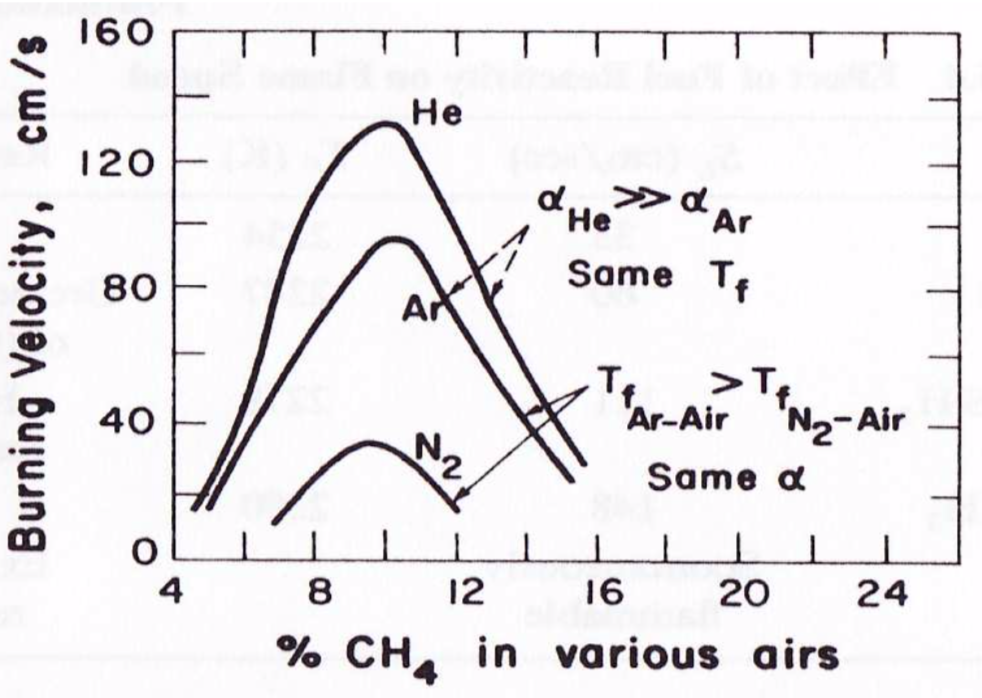
\includegraphics[width=0.6\textwidth]{figures/speed.png}
\end{figure}

\begin{itemize}
    \item $S_{L}$ in $He$ mixture is higher than $Ar$ mixtures. This is due to thermal diffusivity of $He$ which is much larger than that of $Ar$ (because weight of $He$ is much smaller). $He$ and $Ar$ are both monoatomic gas and thus their flame temperature are equal (they have same $C_{p}$).
    \item $S_{L}$ in $Ar$ mixture is higher than $N_{2}$ mixtures. This is due to lower specific heat of $Ar$ ($C_{p}=5/2R$ monoatomic) with respect to $N_{2}$ ($C_{p}=9/2R$ diatomic). But the flame temperature will be higher in the $Ar$.
\end{itemize}

Therefore, high values of $\alpha$ and low values of $C_{p}$ are key for a good burning rate.

\subsubsection{The Burke and Schumann model (D)}

Rather than considering a round jet, the jet is considered to be planar. The geometry is thus totally two-dimensional. Moreover, the jet and the sorrounding air have the same unit flow rate $\rho v$.

\begin{figure}[h!]
\centering
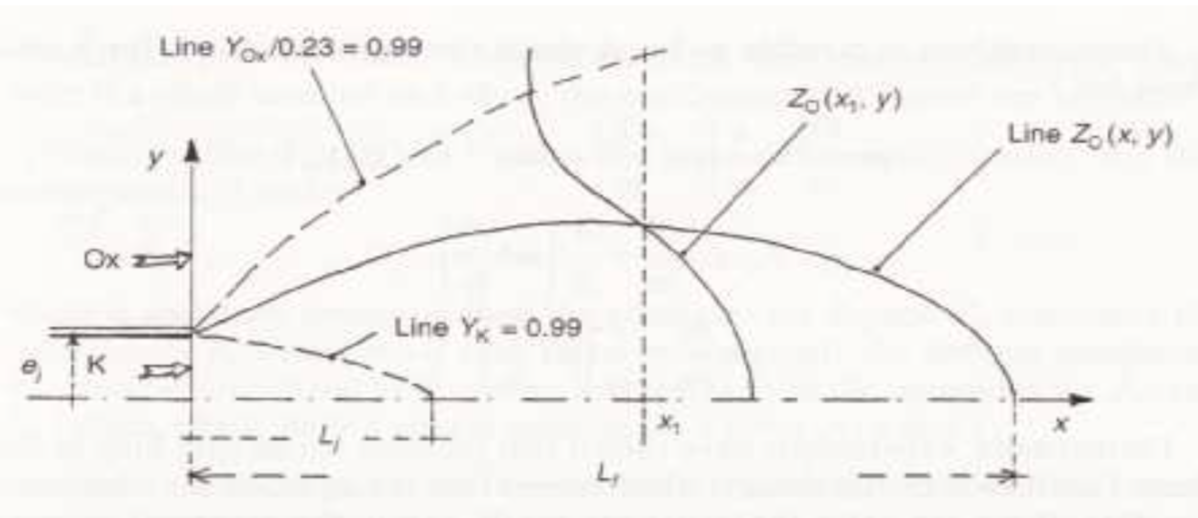
\includegraphics[width=0.8\textwidth]{figures/burke.png}
\end{figure}

Main assumptions:
\begin{itemize}
    \item Steady state
    \item Only three reactive species are present: the fuel ($K$), the oxidant ($Ox$) and the products ($P$).
    \begin{equation}
        K + vOx \rightarrow P
    \end{equation}
    where $v$ is the stoichiometric coefficient
    \item Three equations can be written for $Y_{i}$ where $i=K,Ox,P$
    \item Diffusion is the same: $D_{Ox}=D_{K}=D_{P}=d$
    \item Flow velocity is always parallel to the plane of symmetry, therefore the perpendicular equations are neglected.
\end{itemize}
Under these assumptions the equations are:

\begin{equation}
    \rho v\frac{\partial Y_{i}}{\partial x}=\frac{\partial}{\partial y}\bigg(\rho d \frac{\partial Y_{i}}{\partial y} \bigg) + \rho w_{i}, \text{\;}\text{\;}\text{\;} i=Ox, K, P
\end{equation}
\begin{equation}
    \rho v\frac{\partial h}{\partial x}=\frac{\partial}{\partial y}\bigg(\rho d \frac{\partial h}{\partial y} \bigg)
\end{equation}
\begin{equation}
    \rho v\frac{\partial v}{\partial x}=\frac{\partial}{\partial y}\bigg(\rho d \frac{\partial v}{\partial y} \bigg) - \frac{\partial p}{\partial x}
\end{equation}

Experiments have shown that pressure varies very little in the flame, which means that the last equation become obsolete. The remaining 4 differential equations require boundary conditions at $x=0$, $y=0$, $y=\infty$.\\
Note that since the reaction which consumes K and Ox, is the same as that which produces P, then the rates of reaction by mass for these species are related by their specific stoichiometric coefficients:
\begin{equation}
    \dot{\omega}_{Ox} = v_{s}\dot{\omega}_{K} \text{\;\;\;\;\;\;} \dot{\omega}_{P} = -\dot{\omega}_{K}
\end{equation}
where $v_{s}=v\frac{M_{Ox}}{M_{K}}$ is the mass stoichiometric coefficient.\\
Consequently, if two functions are defined $Z_{0}=Y_{K}-Y_{Ox}/v_{s}$ and $Z_{P} = Y_{K}+Y_{P}$, then these two functions satisfy the following differential equation, obtained as indicated in their definitions:
\begin{equation}
    \rho v\frac{\partial Z_{0}}{\partial x}=\frac{\partial}{\partial y}\bigg(\rho d \frac{\partial Z}{\partial y} \bigg)
\end{equation}
Such functions are called \textit{Schvab-Zeldovitch} functions and they exist only when the diffusion coefficients are the same. They satisfy the boundary conditions. Solving $Z_{0}(x,y)$ is now simply a question of mathematics.

\begin{figure}[h!]
\centering
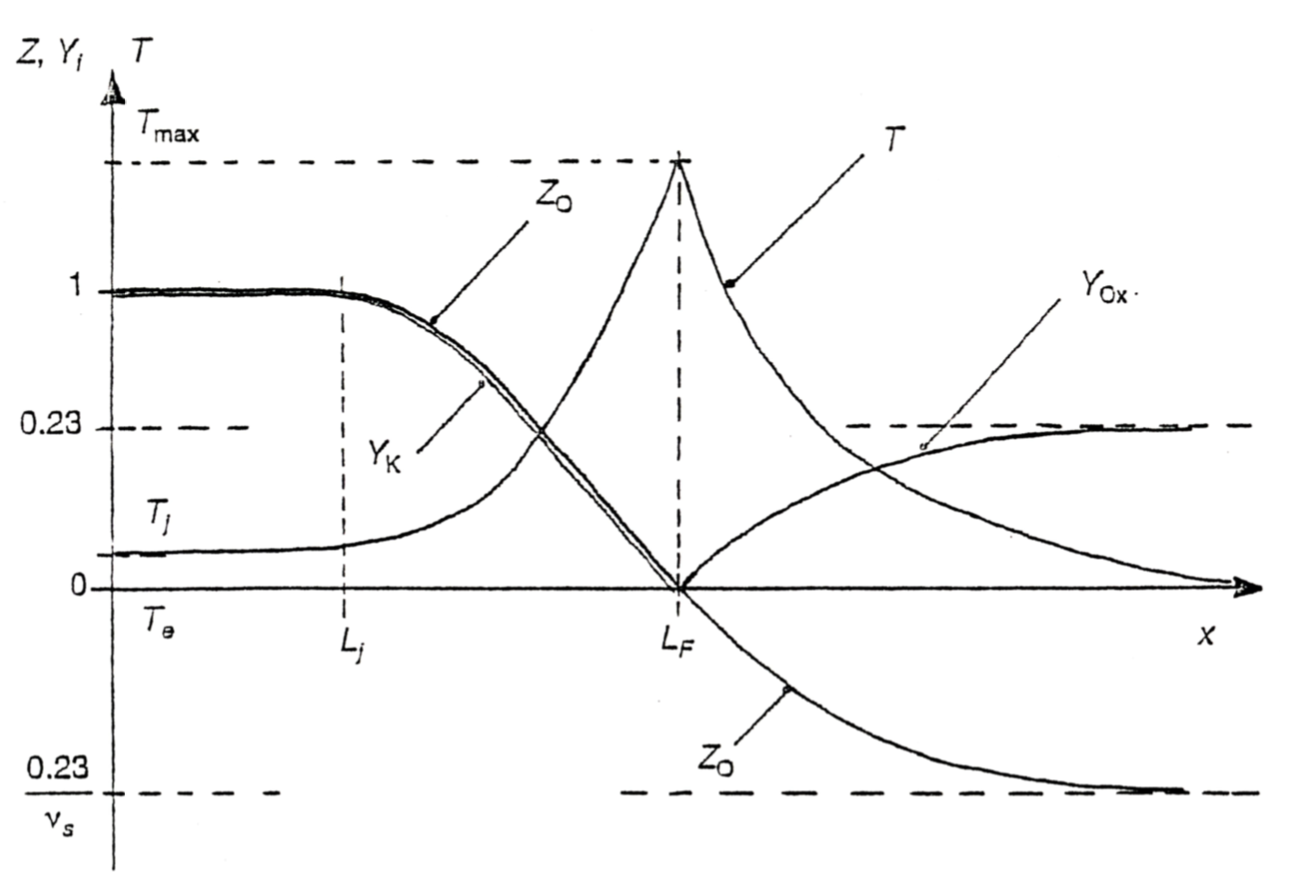
\includegraphics[width=0.6\textwidth]{figures/schumann.png}
\end{figure}

The length of the flame $L_{F}$ is inversely proportional to the diffusion coefficient and the greater is the jet velocity, the longer the flame is.

\subsection{Flame stability}

The stability of a combustion wave can be studied from a flame originated by a Bunsen burner. This is done by analyzing how the position of the flame changes with respect to the outflow section.

\begin{figure}[h!]
\centering
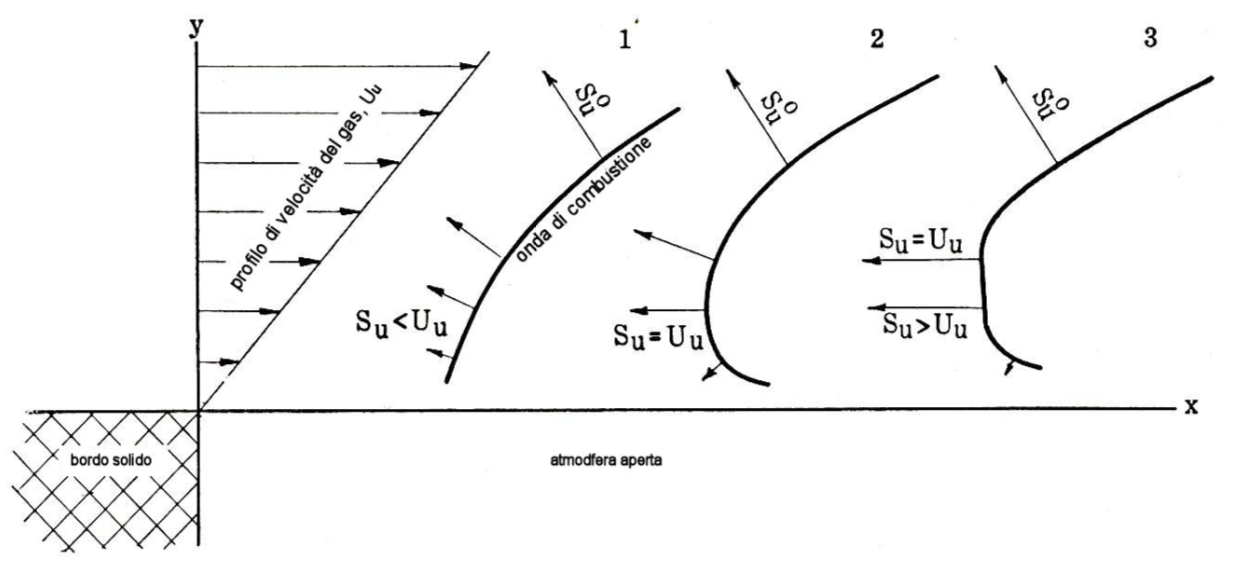
\includegraphics[width=0.6\textwidth]{figures/stability2.png}
\end{figure}

(flow is horizontal)
\begin{enumerate}
    \item combustion wave too close to solid rim. Jet velocity exceeds the flame velocity everywhere ($S_{u}<U_{u}$) and it is pushed back.
    \item equilibrium position ($S_{u}=U_{u}$). Due to the increased distance from the rim the burning rate increases but on the outer part the two velocities are equal.
    \item wave too far from the rim. In some points the flame velocity exceeds the jet and it moves forward toward the equilibrium position.
\end{enumerate}

\subsubsection{Flash-back and blow-off phenomena}

\begin{itemize}
    \item \textit{Flash-back}: upstrean propagation of the flame
    \item \textit{Blow-off}: downstream propagation of the flame
\end{itemize}
These conditions can be characterized by considering the jet and flame velocities and also the distance form the rim.
The parameters to look into to analyze these phenomena is the \textit{velocity gradient}. We can distinguish the critical velocity gradient for flash-back and the critical velocity gradient for blow-off.

\begin{figure}[h!]
\centering
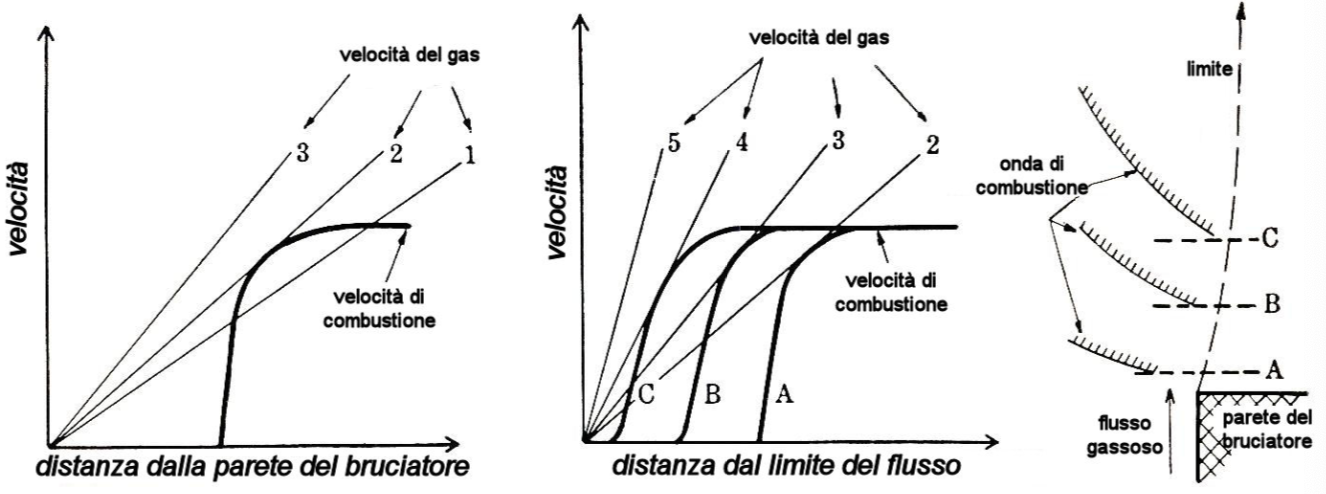
\includegraphics[width=0.9\textwidth]{figures/flash.png}
\end{figure}

\begin{enumerate}
    \item flash-back
    \item flash-back limit
    \item no flash-back
\end{enumerate}

\subsubsection{Quenching for natural gas-air mixtures}

\begin{itemize}
    \item \textit{Quenching}: the distance from the wall in which the flame is unable to propagate under the given conditions.
\end{itemize}
Due to heat transfer from the flame to the walls (which has higher thermal conductivity), temperature of the reaction zone gets lowered below ignition point and the flame gets extinguished.

\begin{figure}[h!]
\centering
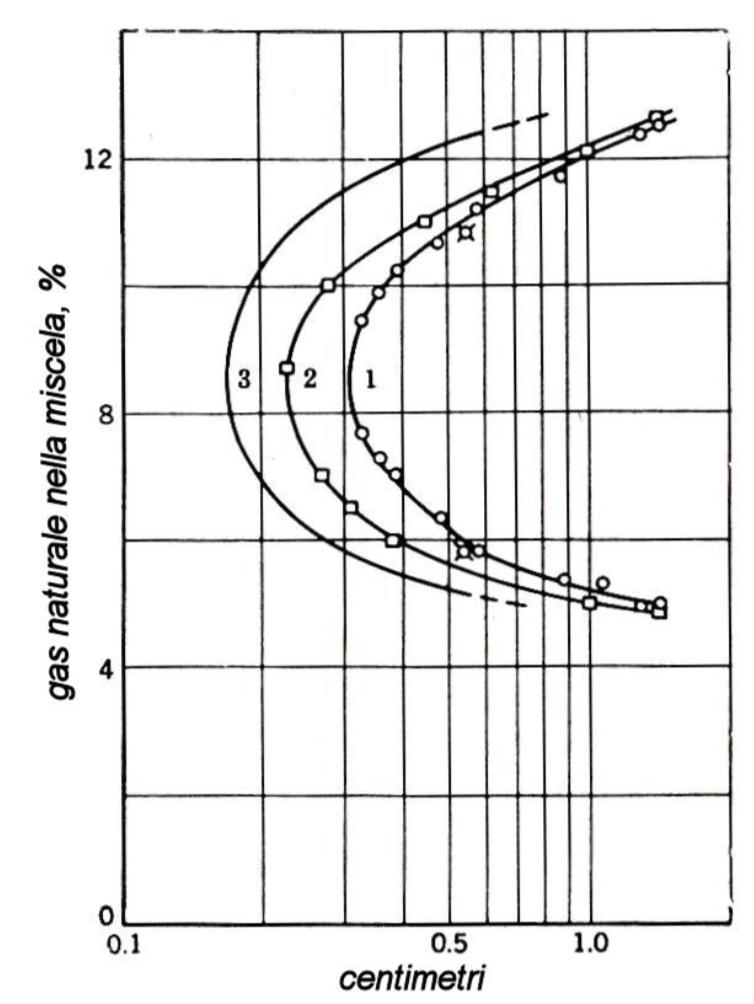
\includegraphics[width=0.4\textwidth]{figures/quenching.png}
\end{figure}

\begin{enumerate}
    \item quenching of cylindrical tubes
    \item quenching between plane-parallel plates
    \item depth of penetration from critical velocity gradient for flash-back
\end{enumerate}

\subsubsection{Characteristic regions of flame stability}

Flame stability is usually characterized by lift-off velocity, lift-off height and blow-out velocity:

\begin{itemize}
    \item \textit{lift-off velocity}: the mean jet velocity at which the flame becomes lifted from the rim exit
    \item \textit{lift-off height}: the distance between the lifted(!) flame base and the rim exit
    \item \textit{blow-out velocity}: the jet velocity at which the reaction cannot be sustained and the flame is extinguished
\end{itemize}

The stability limits of turbulent jet diffusion flames are important for operation of combustion systems and have safety implications. The lift-off and blow-out behaviors have been subject of numerous research efforts to allow the combustion within the stability limits.

\begin{figure}[h!]
\centering
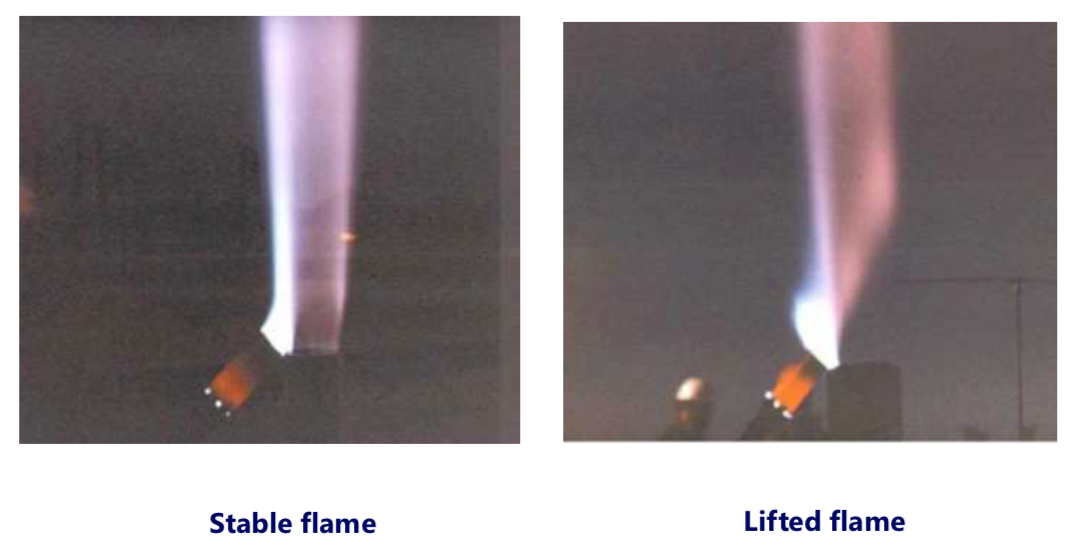
\includegraphics[width=0.5\textwidth]{figures/stableflame.png}
\end{figure}

\begin{itemize}
    \item Stable flame: firmly anchored at the rim exit
    \item Lift-off: permanent separation of the flame from the rim exit
\end{itemize}

\newpage

\section{Ignition and extinction phenomena}

Ignition is a transition from a nonreactive to a reactive state characterized by a self-sustained combustion.\\
The reason for studying ignition is to achieve basic understanding of the detailed process involved. Ignition involve many physical and chemical steps and it is a transient phenomena. Detailed chemical kinetics are used to predict ignition. The usual conditions for ignition are given by a "3T" rule of thumb:

\begin{itemize}
    \item \textit{Temperature}: must be high enough to cause reactions
    \item \textit{Time}: must be long enough enough to allow the heat to be absorbed
    \item \textit{Turbulence}: muste be high enough so that there is good mixing between fuel and oxidizer
\end{itemize}

There are various means of achieving ignition. External stimuli can be classified into:

\begin{itemize}
    \item \textit{thermal energy stimuli}: transfer of energy to the reactants by conduction, convection or radiation
    \item \textit{chemical stimuli}: introduction of \textit{hyoergolic} reactive agents
    \item \textit{mechanical stimuli}: impact, friction or shock wave
\end{itemize}

\subsection{Ignition temperature}

The concept of "ignition temperature" can be inappropiate because the chemical reaction rate is nonzero for all temperatures according to Arrhenius equation. However this concept is still useful.

\begin{itemize}
    \item \textit{van't Hoff ignition temperature}: the temperature at which the rate of heat loss due to conduction is equal to the rate of heat production by chemical reactions
\end{itemize}

\subsection{The thermal ignition}

The rate of heat evolution $q_{r}$ due to chemical reaction in a chamber volume $V$ can be expressed as:
\begin{equation}
    q_{r}=\Delta H_{r} V \dot{\omega} = H_{r} V \bigg[Ae^{\frac{-E_{a}}{R}T} \pi C_{i}^{v_{i}}\bigg]
\end{equation}
where $\Delta H_{r}$ is the heat of reaction and $\dot{\omega}$ is the reaction rate.\\
The rate of heat loss to the walls of a vessel having surface $S$, radius $r_{p}$ and temperature $T_{W}$ can be written as:
\begin{equation}
    q_{L} = -S \lambda \bigg(\frac{\partial T}{\partial r}\bigg) \approx S \lambda\bigg[\frac {(T-T_{W})}{L}\bigg]
\end{equation}
where $\lambda$ is the thermal conductivity and $L$ is the characteristic thickness of the thermal layer near the wall.\\
Both equation depend on the geometry of the vessel, therefore the ignition temperature from these quations will depend upon the geometry.

\begin{figure}[h!]
\centering
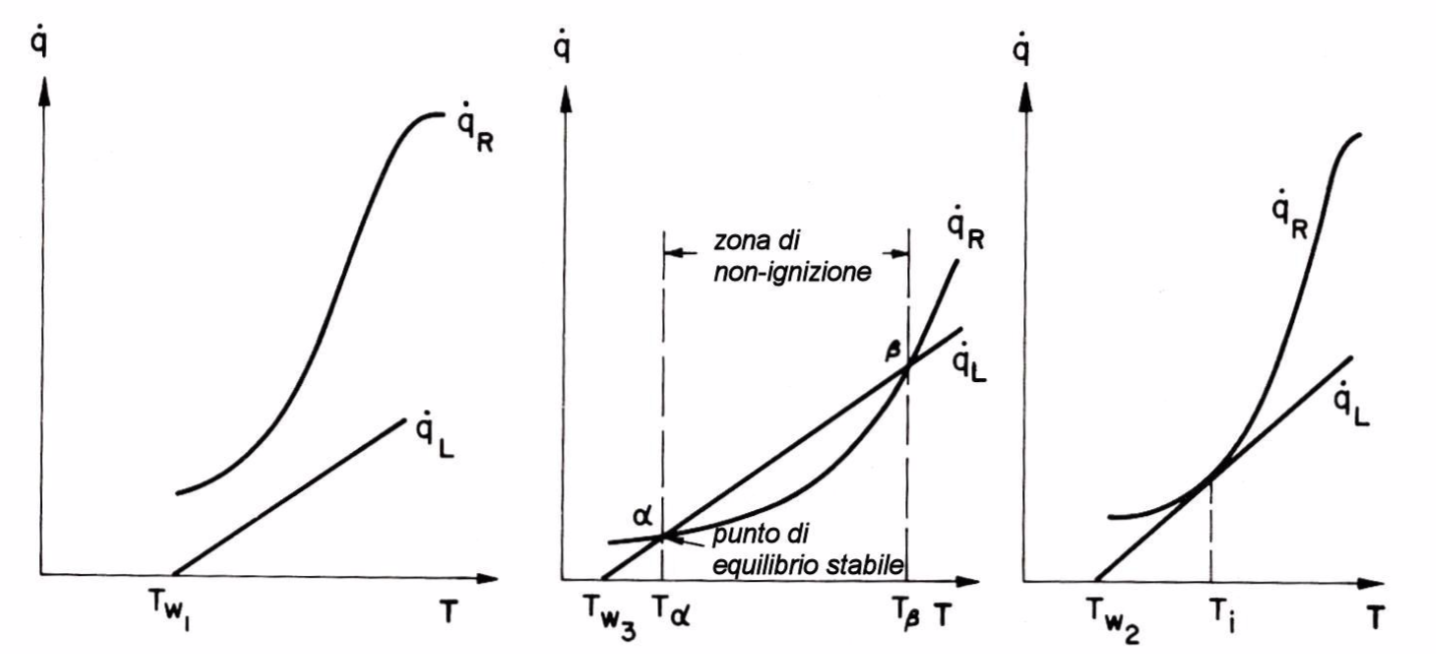
\includegraphics[width=0.6\textwidth]{figures/thermallossgain.png}
\end{figure}

This picture shows the relationship between the heat developed and the heat lost by a mixture in a vessel with temperature controlled walls:

\begin{itemize}
    \item \textit{(left)} the $T_{W}$ is high enough to cause immediate chemmical reactions, in this case $q_{r}$ is always greater than $q_{L}$.
    \item \textit{(center)} the $T_{W}$ is low enough to allow the heat generation by chemical reaction to be significant and the profile of $q_{r}$ near $T_{W}$ is flat. $q_{r}$ intersects $q_{L}$ at $T_{\alpha}$ and $T_{\beta}$. $T_{\alpha}$ is a stable equilibrium point since the mixture will self-heat to $T_{\alpha}$ but no further because $q_{L}$ is greater.
    \item \textit{(right)} the $q_{r}$ curve is tangent to $q_{L}$ at the ignition temperature $T_{i}$. This implies that after the reactants have been introduced into the vessel, they will self-heat to $T_{i}$. $T_{i}$ can be defined mathematically by equating the 2 slopes at the tangent point:
    \begin{equation}
        T_{i}=T_{W}+\bigg(R\frac{T_{W}^{2}}{E_{a}}\bigg)
    \end{equation}
\end{itemize}

\subsection{Effect of various parameters on $T_{i}$}

The effect of chamber volume can be seen from the following figure:

\begin{figure}[h!]
\centering
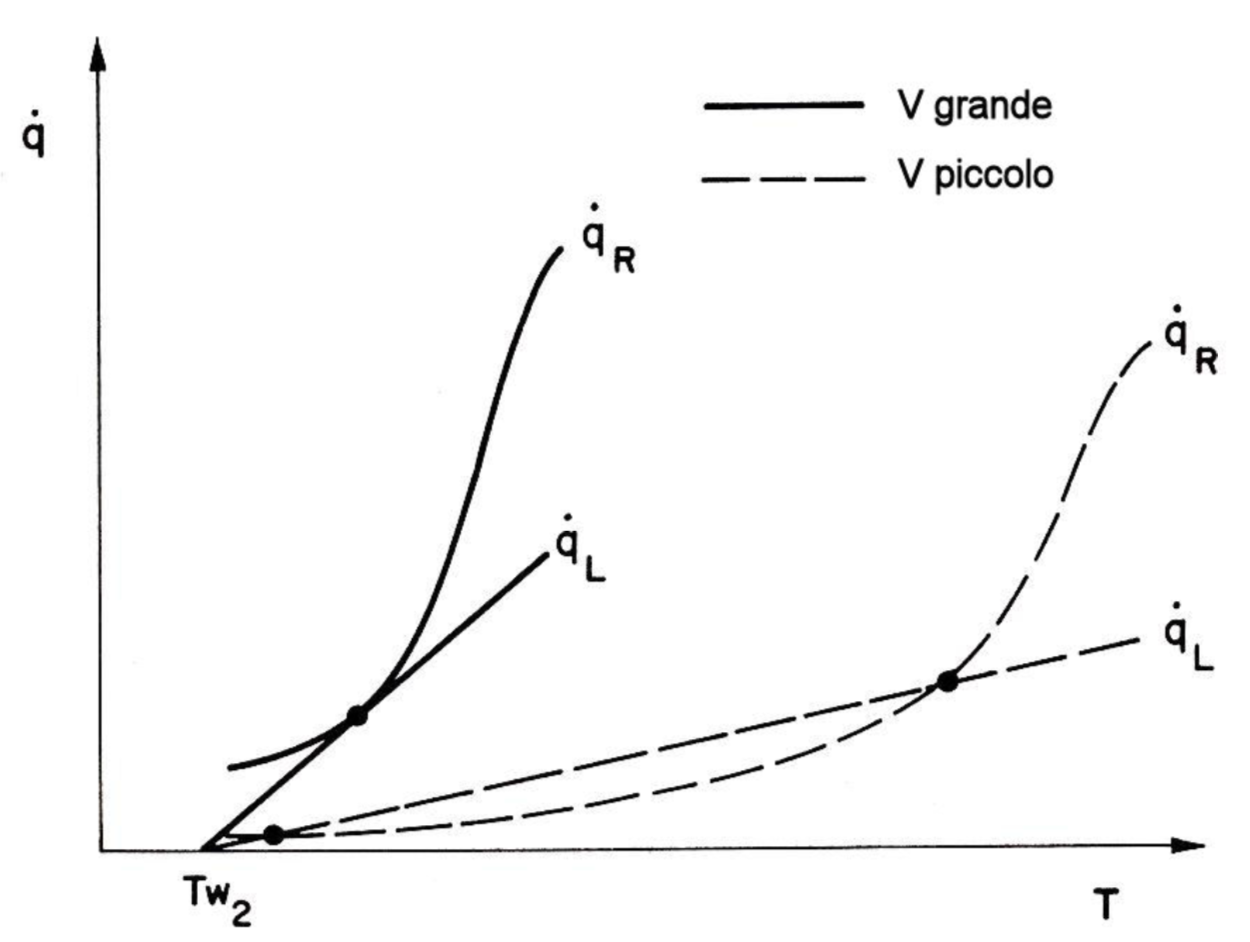
\includegraphics[width=0.5\textwidth]{figures/dashed.png}
\end{figure}

The dashed lines, corresponding to a smaller chamber, show no spontaneous ignition when wall temperature is $T_{W2}$. Thereforem it shows that by decreasing the volume, an ignitable system becomes not ignitable. This is due to the increase of heat loss and reduction of heat developed (see figure).\\
The reactant composition also has an effect on $T_{i}$ since $q_{r}$ is a function of the reaction rate which depends on the composition.\\
In general, $T_{i}$ is a function of:

\begin{itemize}
    \item the size of the apparatus
    \item the initial temperature of the mixture
    \item the reactant composition
    \item the activation energy
    \item time, pressure and turbulence
\end{itemize}

\subsection{Ignition of solid propellants}

The process of combustion of a solid substance involves a more complex analysis:

\begin{itemize}
    \item transfer of energy by conduction, convection or radiation
    \item in-depth energy absorption (inert heating)
    \item decomposition of solid phase, pyrolysis of fuel binder
    \item diffusion of species from the surface
    \item heterogeneous reaction between gaseous species and condensed phase
    \item abrupt increase of temperature
    \item emission of light from the reaction zone
\end{itemize}

\begin{figure}[h!]
\centering
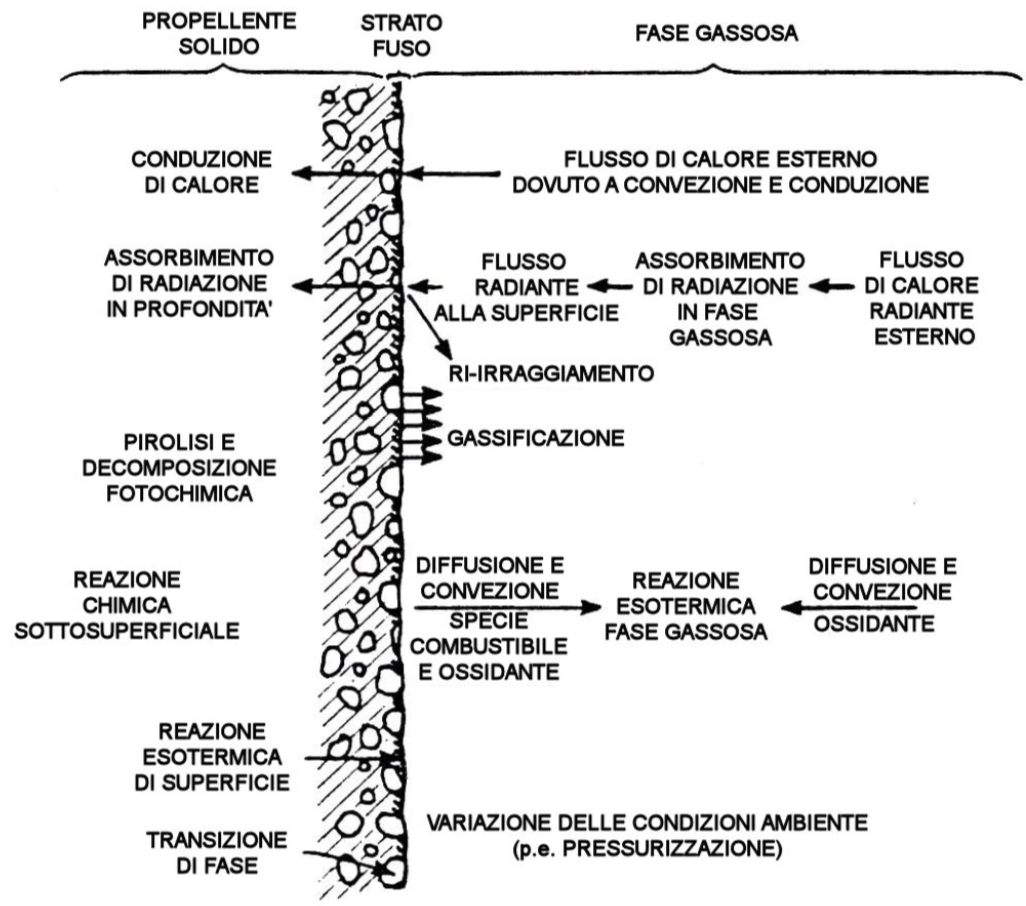
\includegraphics[width=0.6\textwidth]{figures/solid.png}
\end{figure}

\subsection{Ignition phenomena}

When the net heat involved overcomes heat losses, sustained ignition is achieved. Ignition is incomplete of combustion does not follow the ignition event after the removal of stimulus. The time period from the start of the stimulus to the instant of sustained ignition is called the \textit{ignition delay}.\\
Ignition theories are classified into 3 groups:

\begin{itemize}
    \item \textit{gas phase}: considers the ignition process to be controlled by the reaction between the fuel and oxidizer mixtures and the ambient oxidizer gases
    \item \textit{heterogeneous}: considers the reaction between the solid-phase fuel and ambient oxidizer at the interface
    \item \textit{solid-phase}: does not consider heat release and mass diffusion in the gas phase. The temperature rise inside a solid propellant is achieved by the heat release caused by subsurface reactions or external heating.
\end{itemize}

Within the 3 theories described above, several models have been proposed. These models differ in the governing equations considered, assumptions made, ignition criteria and type of propellants studied.

\subsection{Explosion limits}

\begin{figure}[h!]
\centering
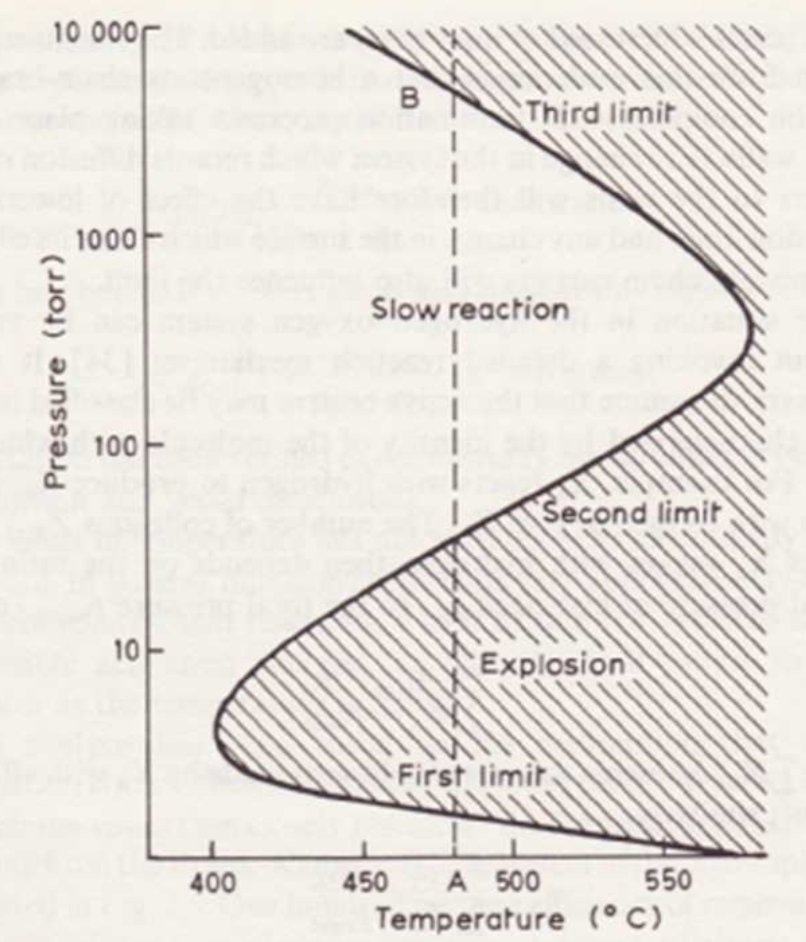
\includegraphics[width=0.4\textwidth]{figures/explosion.png}
\end{figure}

\begin{itemize}
    \item \textit{First limit}: the lower limit is affected by the nature of the surface coating of the container
    \item \textit{Second limit}: this limit is considered at higher pressures. At this limit, an increase in pressure inhibits the explosive reaction
    \item \textit{Third limit}: the rate of reaction is usually quite high immediately below the third limit and the characteristic observed tend towards those associated with thermal explosion
\end{itemize}

\subsection{Ignition of keresone sprays}

\begin{figure}[h!]
\centering
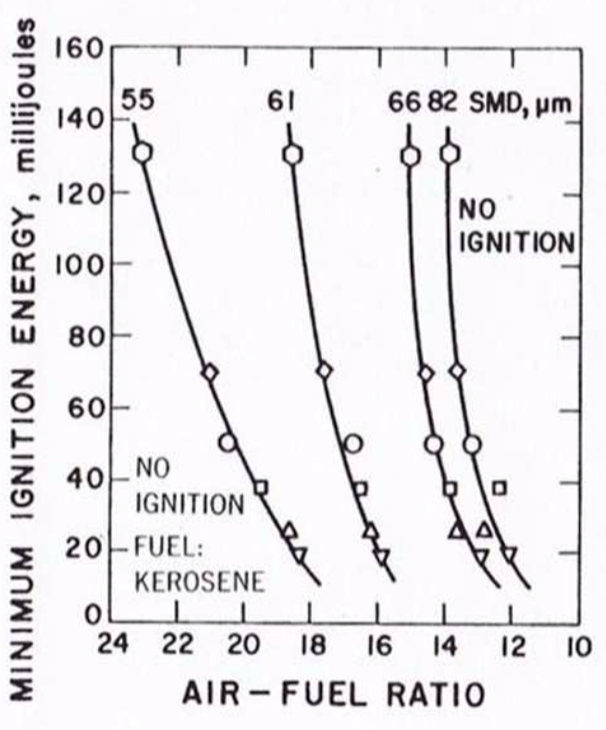
\includegraphics[width=0.3\textwidth]{figures/kerosene.png}
\end{figure}

The minimum ignition energy is plotted for 4 different values of the mean drop size. For each curve the left-hand size represents a region of no ignition and the right-hand size a region of ignition. This figure shows how the weak-ignition limit is improved by a reduction of drop size. The curves become steeper with increasing the drop size which indicates that a much greater increase in spark energy is needed.

\begin{figure}[h!]
\centering
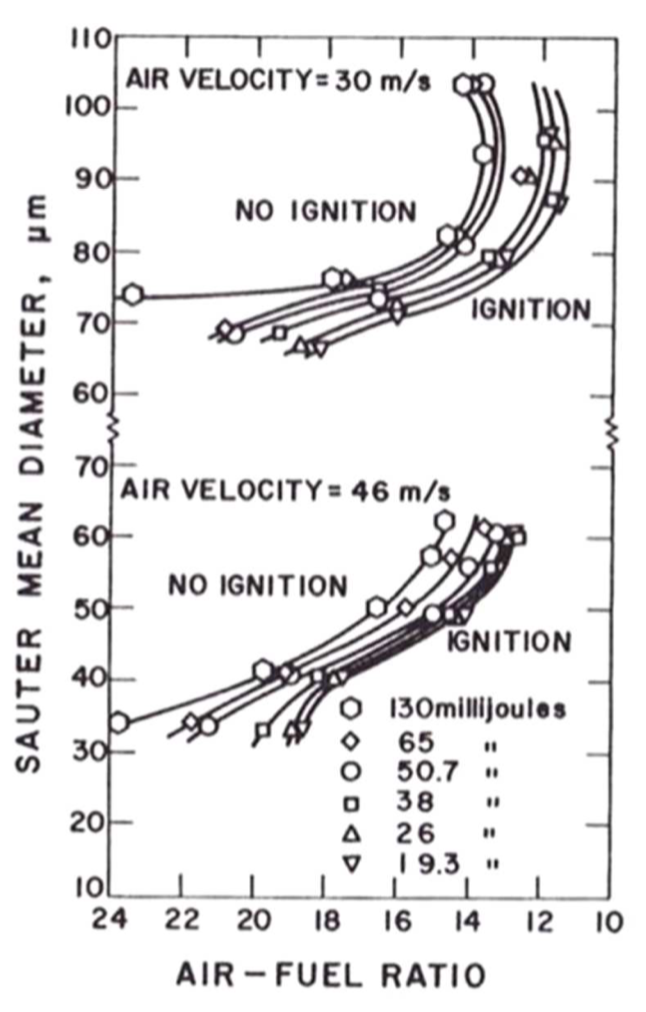
\includegraphics[width=0.3\textwidth]{figures/kerosene2.png}
\end{figure}

In this figure the ignition limits obtained at 2 different air velocities are plotted in terms of \textit{SMD} (sauter mean diameter - average of particle size) vs air-fuel ratio. For both velocities the weak-ignition limits are widened by an increase in spark energy. As the air-fuel ratio is reduced towards the stoichiometric value ($14.8$), the more rapid reaction releases more heat that allows further fuel evaporation and extend the ignition limits into a region of larger drop sizes.

\begin{figure}[h!]
\centering
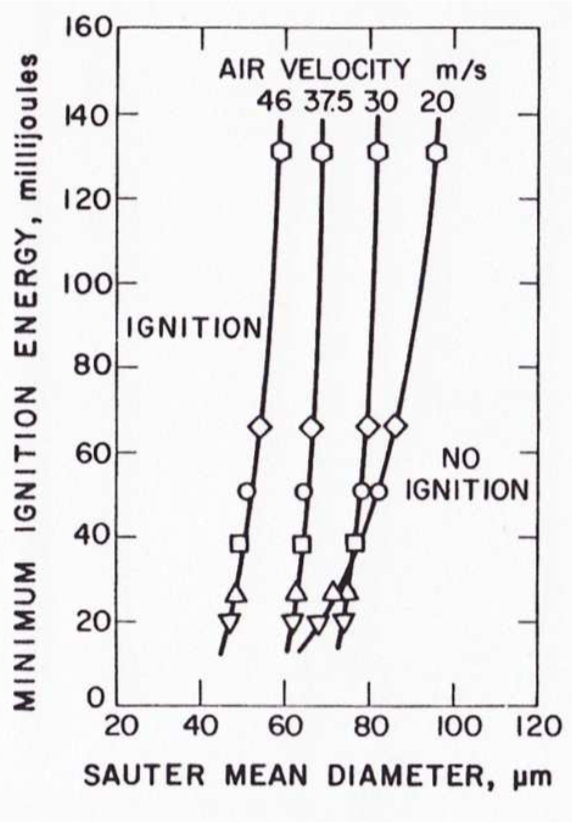
\includegraphics[width=0.3\textwidth]{figures/kerosene3.png}
\end{figure}

The figure shows the variation of minimum ignition energy vs the SMD for stoichiometric mixtures at 4 velocities. At all values of velocity, large increases in spark energy are needed to compensate for quite modest increase in drop size. This figure illustrates the crucial role of the fuel injector in the attainment of good ignition performance. Moreover improvements in the atomization during the ignition and minimization of the flow velocity (reduction of speed is good) in the ignition zone can significantly enhance ignition of sprays in flowing air streams.

\subsubsection{Minimum ignition energy}

The least amount of energy required from an external source to create such a spark whose size is equal to the quenching distance is defined as the \textit{minimum ignition energy $E_{min}$}:

\begin{equation}
    E_{min} = C_{p, air}\rho_{air}\Delta T_{stoich} \frac{\pi}{6}d_{q}^{3}
\end{equation}

the results of these experiments show that the most important parameters affecting $E_{min}$ are drop size, air velocity and fuel-air ratio. In particular, even a slight improvement in atomization quality decreases $E_{min}$ and is beneficial to ignition.

\newpage

\section{Two-phase flow combustion}

\subsection{Droplet combustion}

The simplest case to study is not that of a drop whose diameter reduces as it burns, but rather that of a drop which is fed with fuel at its center so the diameter remains constant. With this arrangement the problem is stationary, the flame and the drop can be described with one spatial variable, the distance from the center of the drop.\\
The combustion of a single droplet is studied using the double-film model. One film separates the droplet surface from the flame front, and the other separates the flame from the sorrounding oxidizer.

\begin{figure}[h!]
\centering
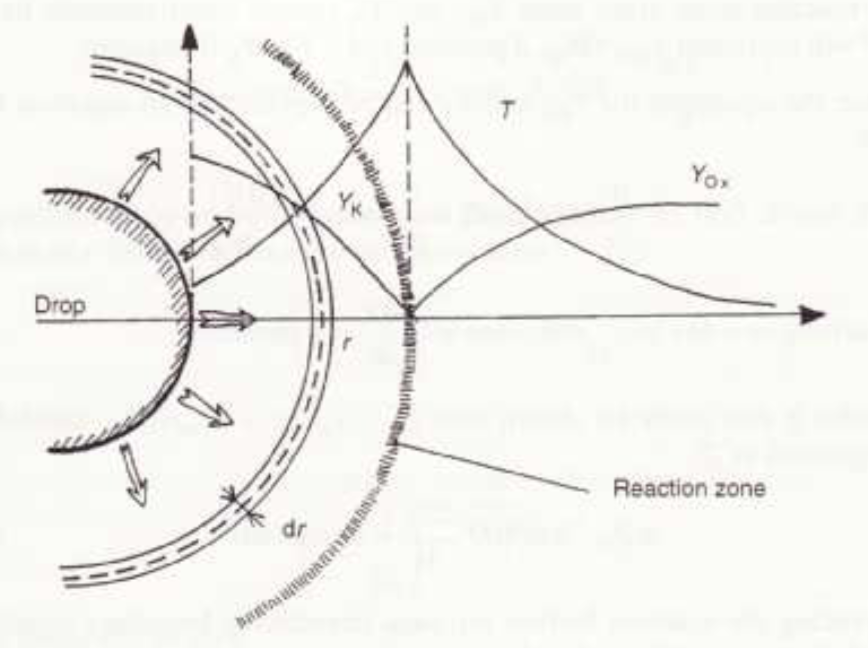
\includegraphics[width=0.5\textwidth]{figures/droplet.png}
\end{figure}

The solution of this problem is performed using the following assumptions:

\begin{itemize}
    \item pressure is constant
    \item the drop is at uniform temperature
    \item the $C_{p}$ for the gas is constant
    \item an infinitely rapid chemical reaction of the type $K+vOx \rightarrow P$ occurs
    \item the coefficient of molecular diffusion for $Ox$ and $K$ are all equal to $D$, and $\rho D$ can be assumed constant
\end{itemize}

The most important parameter to consider is the \textit{mass burning rate} since it permits the evaluation of the \textit{evaporation coefficient}.

\subsubsection{The evaporation coefficient}

The evaporation coefficient $\beta$ is defined by the following $d^{2}$ evaporation law:
\begin{equation}
    d^{2}=d_{0}^{2}-\beta_{0}t
\end{equation}
where $d_{0}$ is the original drop diameter, amd $d$ the drop diameter after time $t$.\\
We are interested in the rate of regression of he condensed material (mass consumption). The condensed phase must be gasified, and consequently there must be an energy input into the condensed material. The heat of flux at the surface determines the rate of regression:
\begin{equation}
    q_{s}=r\rho_{liq}Q
\end{equation}
(s: surface)
\begin{itemize}
    \item $q_{r}$ is the heat flux to the surface
    \item $r$ is the regression rate
    \item $Q$ is the energy required to bring the material to the temperature of vaporization
\end{itemize}

\subsubsection{Evaporation of a single fuel droplet}

The fuel \textit{evaporation rate} expression can be written as:
\begin{equation}
    G_{F}=\frac{\dot{m}_{F}}{4\pi r_{s}^{2}}=\rho_{s}\mathcal{D}_{s}\frac{ln(1+B)}{r_{s}}
\end{equation}
 where $B$ is called the \textit{Spalding transfer number}:
 \begin{equation}
     B=b_{\infty}-b_{s}=\frac{Y_{Fs}-Y_{F\infty}}{1-Y_{Fs}}
 \end{equation}
 The value of $B$ must be evaluated in order to calculate the mass evaporation rate. Before that, $Y_{F}$ (fuel mass fraction) or $p_{F}$ must be determined, but the gas which sorrounds the droplet is saturated by the vapor or liquid of the droplet at the surface. Thus the problem becomes to determine $T_{d}$ since pressure data are available.\\
 The time of evaporation of a liquid droplet is an important parameter in combustion chamber design since the lifetime of the largest droplet in a spray determines the minimum time the droplet must be allowed to reside in the combustion chamber.
 
\begin{figure}[h!]
\centering
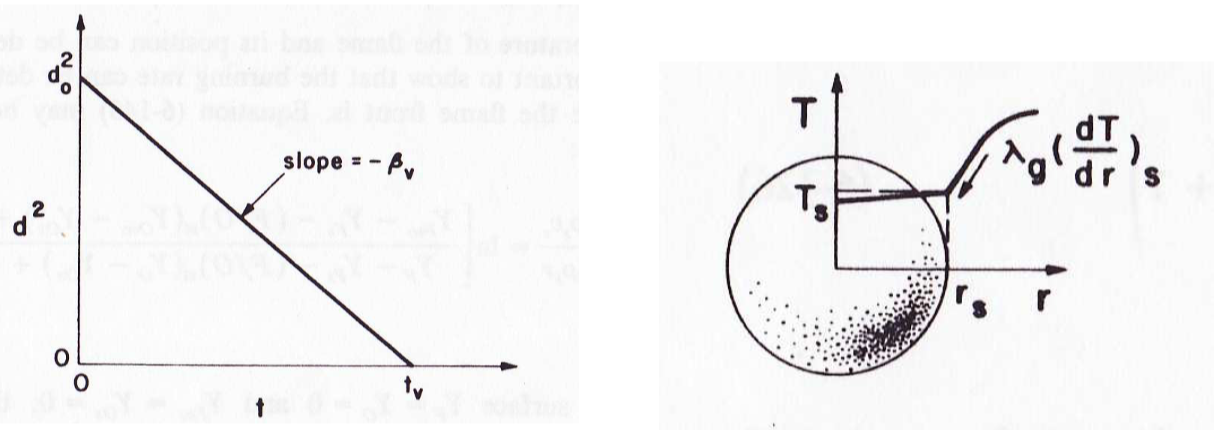
\includegraphics[width=0.8\textwidth]{figures/droprate.png}
\end{figure}

\begin{itemize}
    \item (left) the $d^{2}$ evaporation law for liquid fuel droplets. Note that the evaporation coefficient $\beta$ represents the magnitude of the negative slope
    \item (right) the temperature distribution of an evaporating liquid droplet
\end{itemize}

\begin{figure}[h!]
\centering
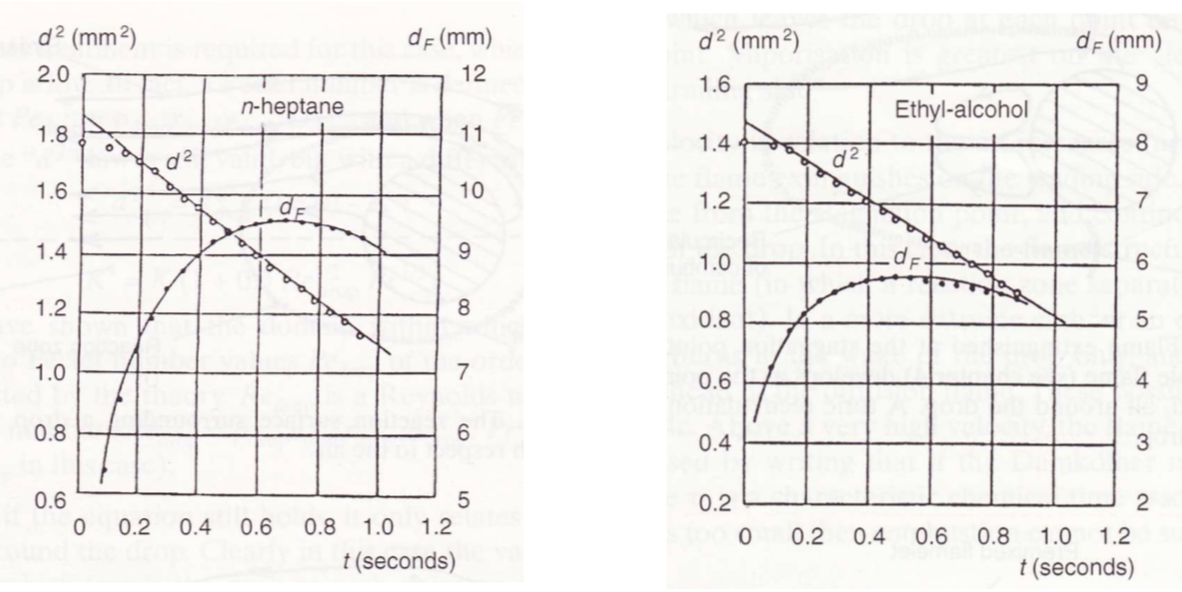
\includegraphics[width=0.8\textwidth]{figures/flamediameter.png}
\end{figure}

Note that the ratio $\frac{r_{F}}{r_{drop}}$ ($r_{F}$ is the radius of flame) assumed to be constant in the steady-state theory, varies greatly as the drop burns. This is apparent in the figure which plots the diameters.

\subsubsection{Combustion of a single fuel droplet}

In a single droplet burning analysis we assume that the fuel and oxidant depletion rates are related in stoichiometric proportions:
\begin{equation}
    \dot{\omega}_{F} = \dot{\omega}_{0}(F/O)_{stoich}
\end{equation}

TODO

\subsection{Spray combustion systems}

Spray combustion occurs in liquid rocket engines, gas turbines, diesel engines. The predictive models for spray combustion processes becomes important. A realistic analytical model of a combusting spray must involve consideration of several phenomena such as:
\begin{itemize}
    \item spray formation and transport characteristics of individual droplets
    \item turbulent two-phase flow
    \item interactions of radiation with flame turbulence
\end{itemize}

Sprays are burned in various ways, and each poses different problems:

\begin{figure}[h!]
\centering
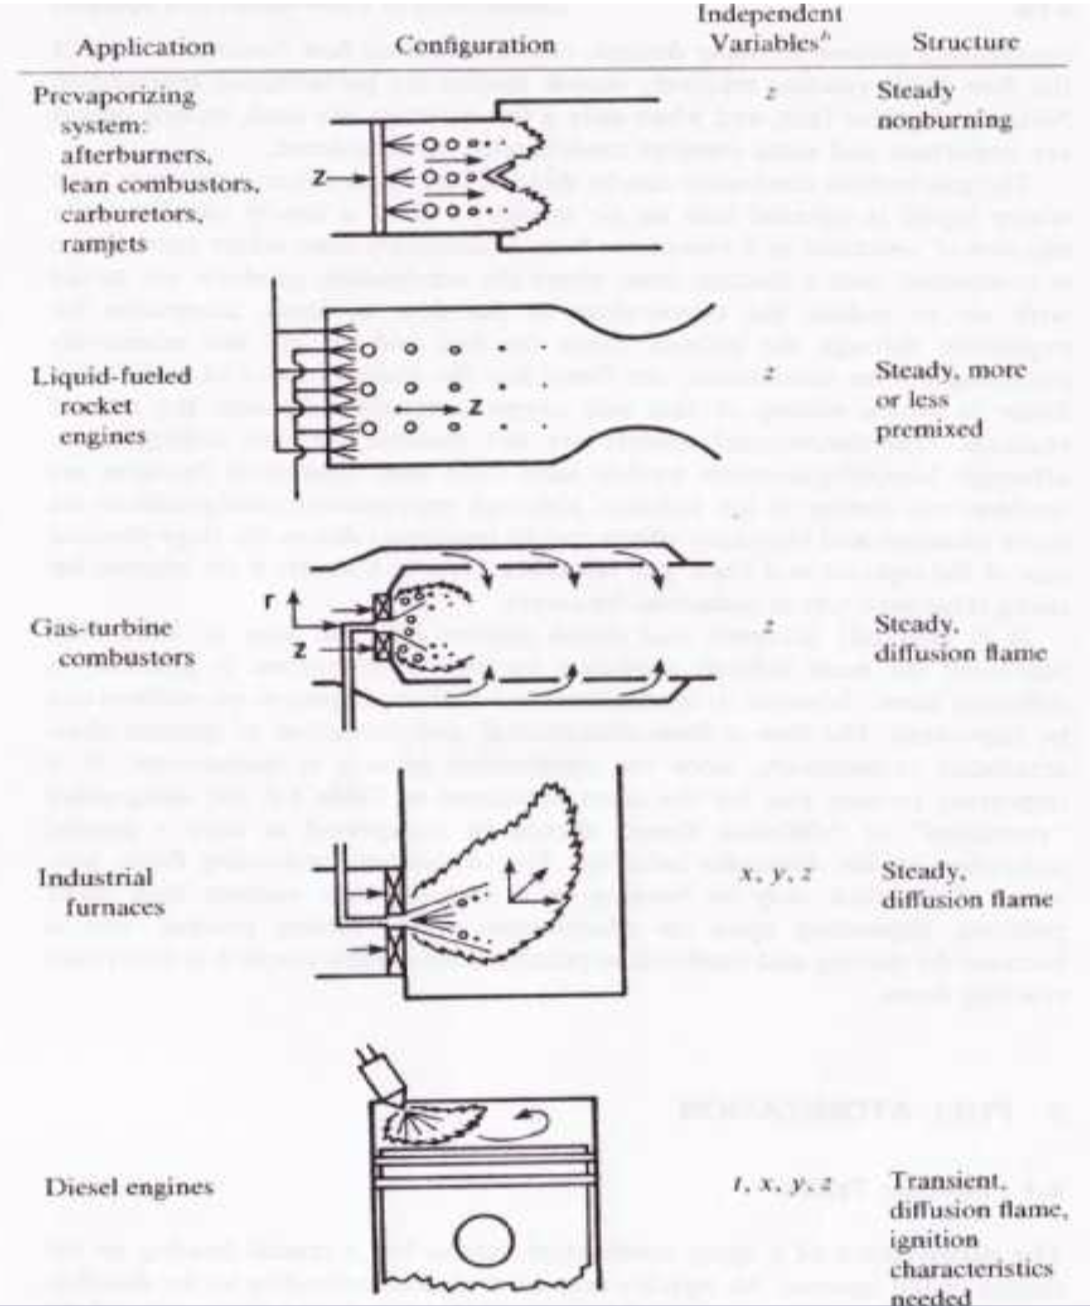
\includegraphics[width=0.4\textwidth]{figures/spraycomb.png}
\end{figure}

\begin{itemize}
    \item \textit{prevaporizing system}: the spray is injected in a heated air stream and the drops are almost completely evaporated before reaching the flame (afterburners)
    \item \textit{liquid rocket engines}: both fuel and oxidizer are injected from one end, providing a more or less premixed
    \item \textit{gas turbine combustor}: the fuel and air are not extensively premixed before combustion, the flame has the characteristics of a diffusion flame
    \item \textit{industrial furnaces}: similar to gas turbines
    \item \textit{diesel engines}: the process is primarily a diffusion flame, prediction is necessary since the combustion process is intermittent
\end{itemize}

\subsubsection{Fuel atomization}

Injectors can be classified into 2 categories:

\begin{itemize}
    \item \textit{pressure-atomizing injectors}: atomization is achieved by pressure drop
    \item \textit{twin-fluid injectors}: atomization of the liquid is aided by a flow at high velocity through injector passages
\end{itemize}


\subsubsection{Spray particles characterization}

The shape of liquid droplets may be considered to be spherical (can be characterized by only the radius) when the following 2 conditions are met:
\begin{enumerate}
    \item the collision and agglomeration effects are small, this requires that the volume occupied by the condensed phase be much less than the total spatial volume
    \item the \textit{Weber} number is low ($We<20$), the degree of deformation of a droplet caused by the slip velocity between the droplet and gas depends upon the ratio of the dynamic force to the surface-tension force:
    \begin{equation}
        We = \frac{dynamic force}{surface tension force} = 2r\rho_{gas}\frac{(v_{drop}-v_{gas})^{2}}{\sigma_{s}}
    \end{equation}
\end{enumerate}

\subsubsection{Drop size distribution}

Overall spray characteristic are represented by distribution curves which are given in terms of the cumulative percentage. In many processes it is desirable to work only with average diameters instead of the complete drop-size distribution.

\begin{figure}[h!]
\centering
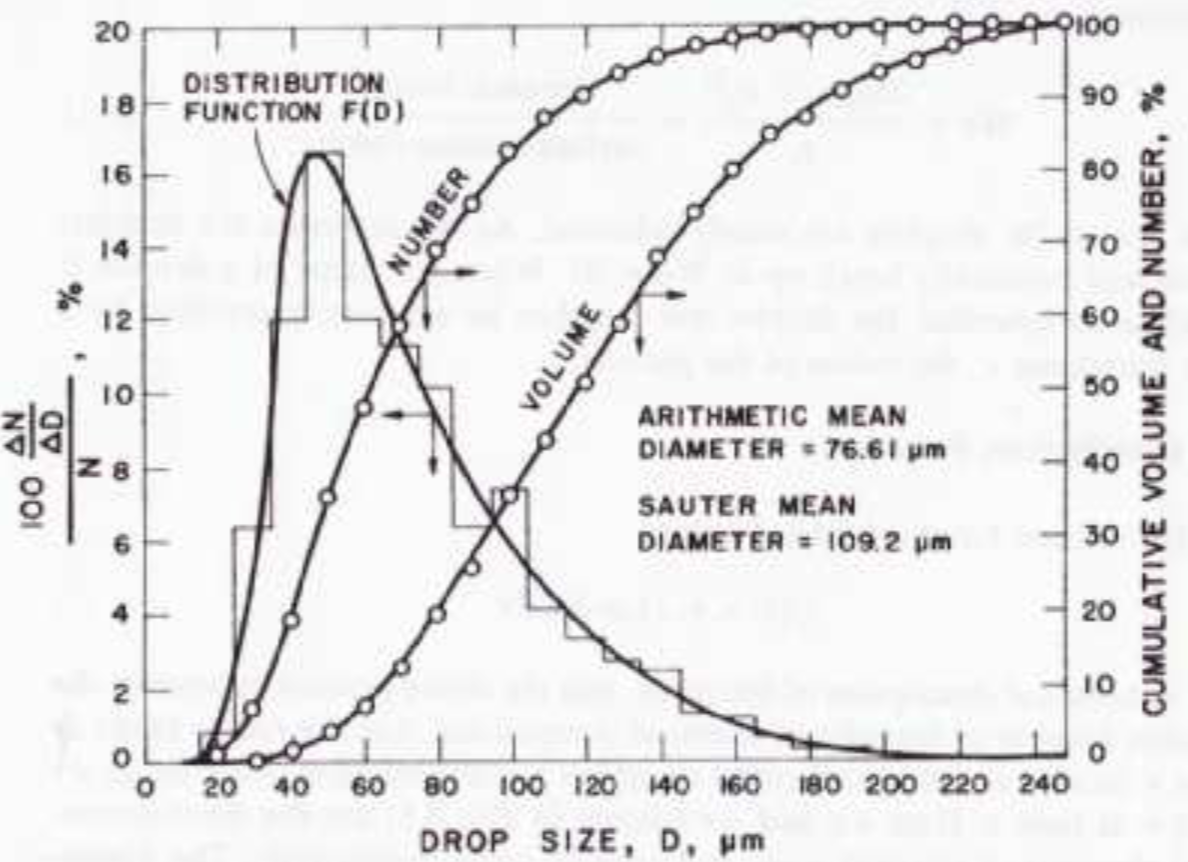
\includegraphics[width=0.4\textwidth]{figures/distribution.png}
\end{figure}

\subsubsection{Spray combustion characteristics}

Although combustion of droplets in a spray in governed by the diffusion of fuel vapor and oxidizer, both premixed and diffusion flame theories have been applied to spray combustion problems but for the former caution must employed.\\ For both cases, it must be considered the size and volatily of the droplet since for very small droplets of a high-volatily fuel, the droplet evaporation may be completed in the heat-up process, so that the flame structure is not influenced by the two-phase flow.

\subsubsection{Spray and gas flame comparison}

Experiments on spray combustion flames of axial jets of kerosene show the region where the droplets exist is limited to a small area above the burner nozzle. It is concluded that most of the droplets in the flame do not burn individually but that fuel vapor from the droplets forms a cloud and burns like a gaseous diffusion flame.\\ Changing only the fuel from liquid kerosene to gaseous propane, the spray combustion flame was found to be very similar to the previous. It is obvious that there is a resemblance between the two cases. However in the gas diffusion flame, chemical reactions occured slightly downstream as compared with the spray one. This is due to higher flow velocity of propane than of kerosene. In the spray, the temperature drop in steeper than in the gas diffusion flame, the difference is caused by the higher radiation cooling rate of the spray combustion flame.

\begin{figure}[h!]
\centering
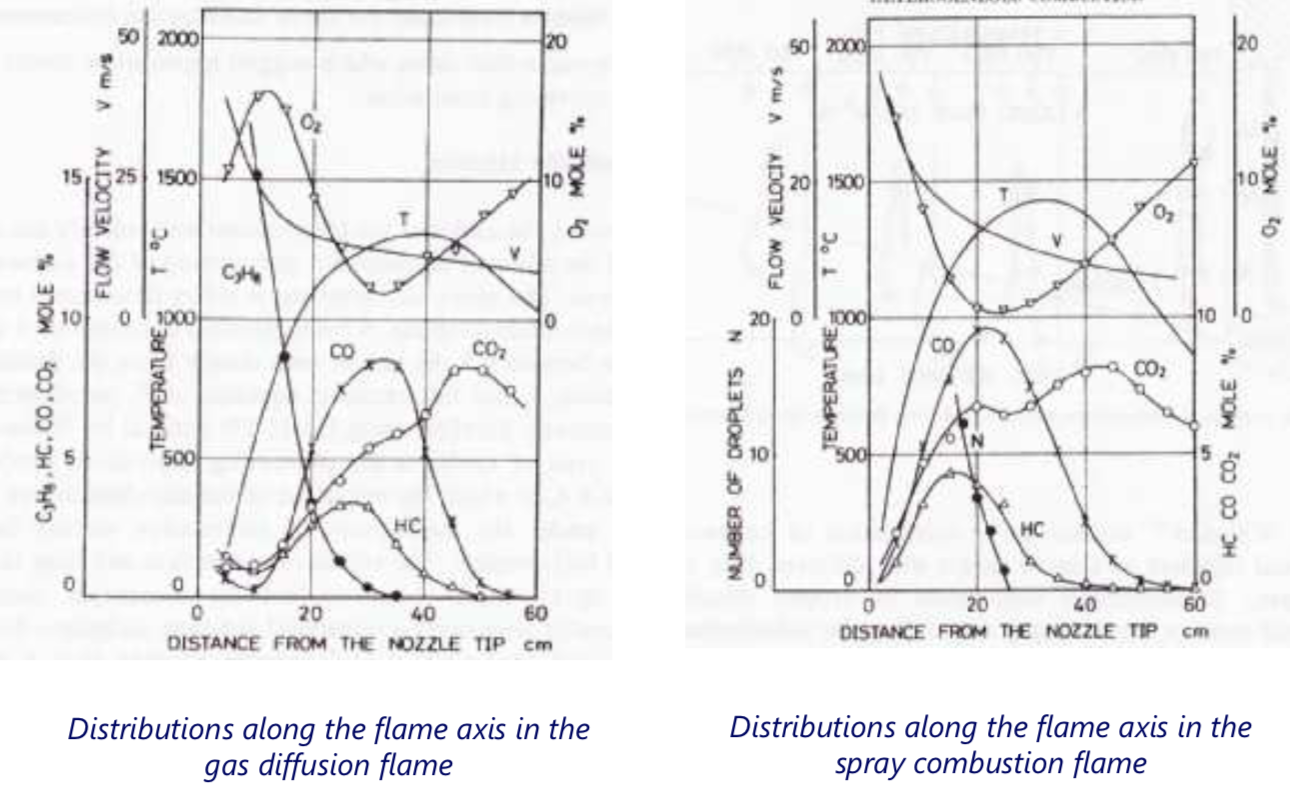
\includegraphics[width=0.6\textwidth]{figures/spraygas.png}
\end{figure}

\subsubsection{The spray combustion process}

\begin{figure}[h!]
\centering
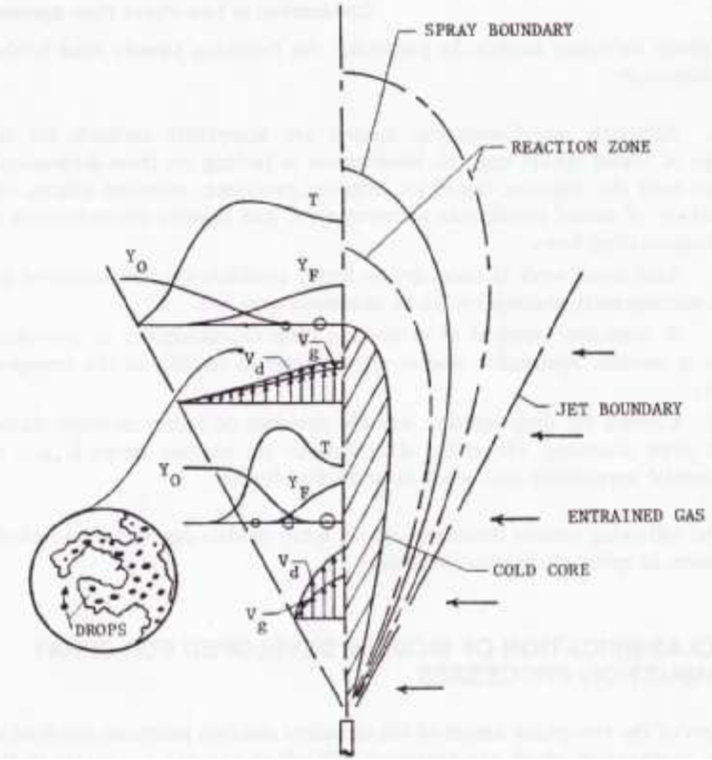
\includegraphics[width=0.5\textwidth]{figures/core.png}
\end{figure}

The figure illustrates the locations of the cold core region, reaction zone, spray boundary and jet boundary of a coaxial spray diffusion flame. The spray leaving the injector is highly nonuniform with smaller droplets at the periphery and larger droplets near the centerline. The outer small droplets evaporate rapidly to provide fuel vapor which is consumed near the outer portion of the turbulent diffusion flame. Larger droplets can travel long distance before evaporation and combustion processes begin, this is due to the high inertia. With increasing distance from the injector exit, the centerline temperature increases due to combustion of the spray. Experiments show that the disappearance of droplets is correlated with positions of maximum temperature, instead fuel evaporation occurs in relatively cool regions.

\subsection{Spray combustion in a Diesel reciprocating engine}

The goal is to develop predictive combustion models for diesel engines. Today, models are able to predict the \textit{ignition delay} including $NO$ and $soot$ emissions. Diesel combustion models can be classified into 2 groups:
\begin{enumerate}
    \item \textit{thermodynamic models}: aim to calculate the heat release rate according to a given pressure history
    \item  \textit{multidimensional models}: are based on the evaluation of the fluid dynamic properties such as temporal and spatial variations, composition, pressure and turbulence. They are more predictive and can provide more fundamental information of the combustion phenomena
\end{enumerate}

\subsubsection{KIVA-II}

KIVA-II is a program devoted to the numerical calculation of transient, 2 and 3-dimensional reactive fluid flows with sprays. A stochastic particle model is used to calculate evaporating liquid sprays, including the effects of droplet collisions.\\
The in-cylinder dynamics of internal combustion engines involve complex physical and chemical processes. These include the transient 3-dimensional dynamics of evaporating fuel sprays, chemical reactions and heat transfer. The KIVA code has the ability to calculate such flows with arbitrarily shaped piston geometries and it solves the unsteady equations of motion of the reactive mixture coupled to the equations for a single component vaporizing fuel spray.\\
The KIVA equations can be used to solve both laminar and turbulent flows which differ primarily in the form and magnitude of the transport coefficients (much larger in the turbulent case).

\begin{figure}[h!]
\centering
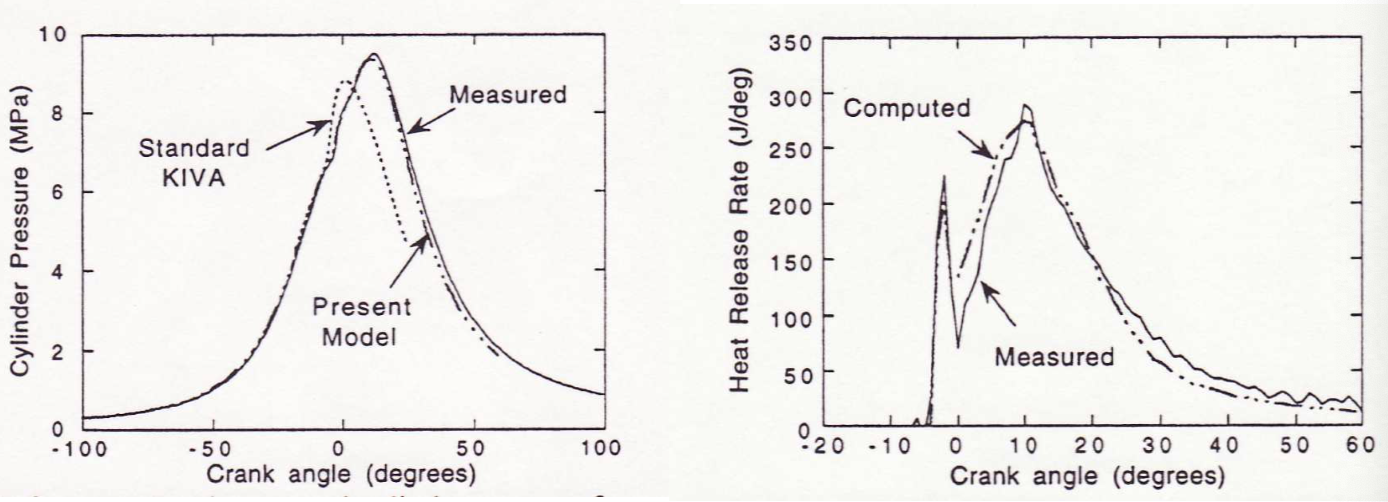
\includegraphics[width=0.6\textwidth]{figures/kiva.png}
\end{figure}

The figures show the computed and measured cylinder pressure (left) and the computed and measured heat release (right) for a Caterpillar engine.

\begin{figure}[h!]
\centering
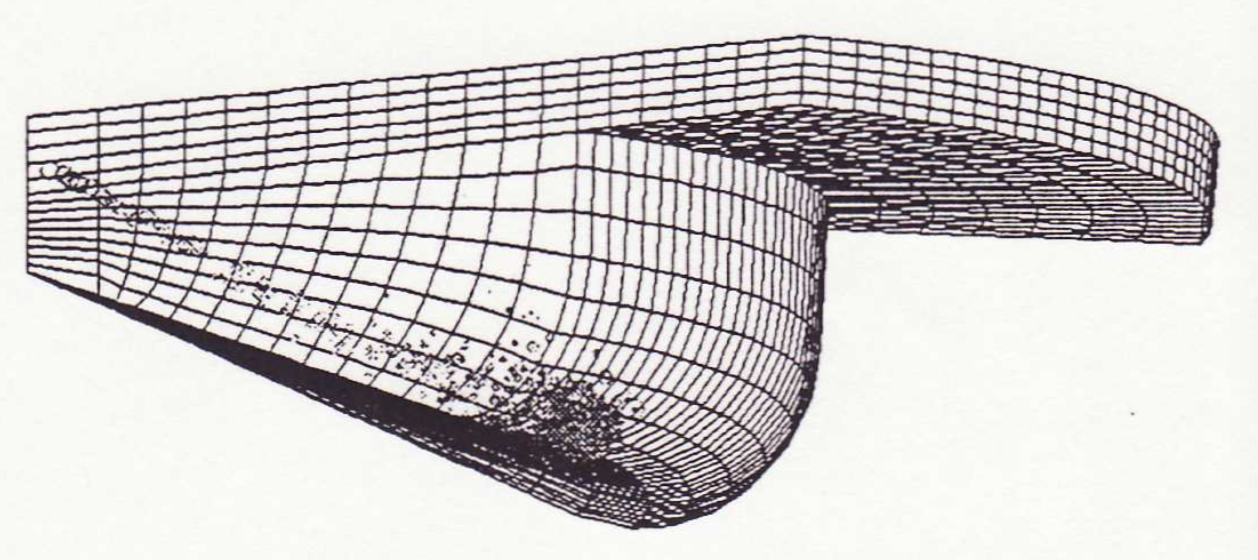
\includegraphics[width=0.4\textwidth]{figures/grid.png}
\end{figure}

Perspective view (1/6 of the combustion chamber) of the computational grid and fuel droplet distribution.

\begin{figure}[h!]
\centering
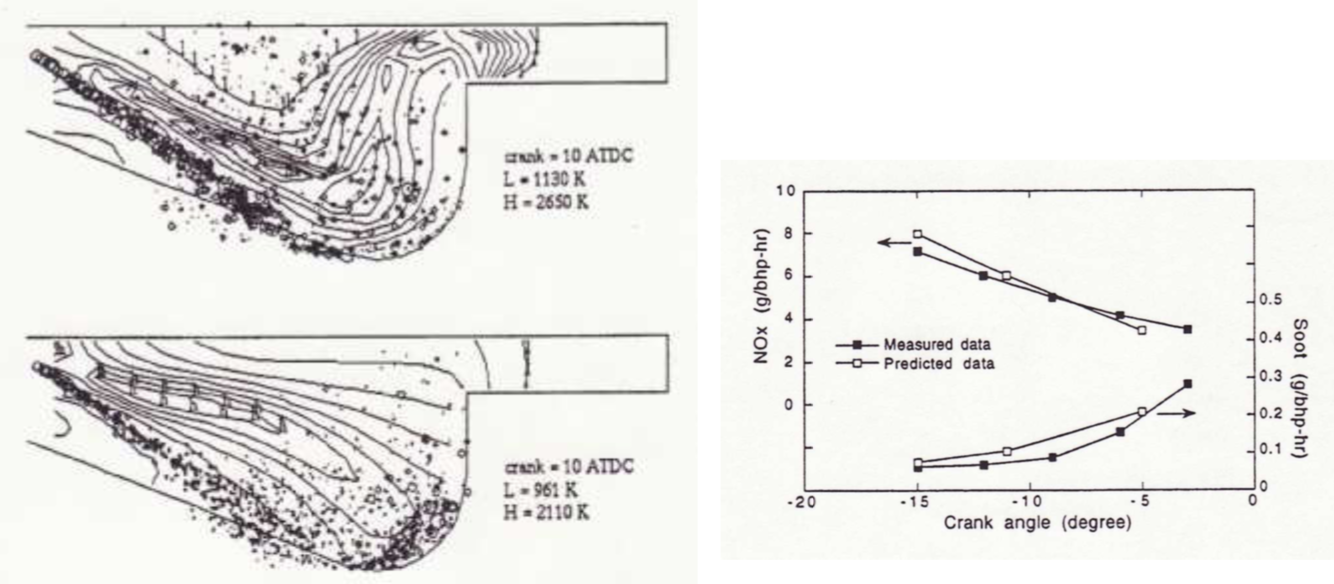
\includegraphics[width=0.6\textwidth]{figures/kiva2.png}
\end{figure}

In-cylinder gas temperature contours computed using different models (left), the wall impingement is visible. Comparison between computed emissions and measured engine-out data with varying fuel injection timing.

\begin{figure}[h!]
\centering
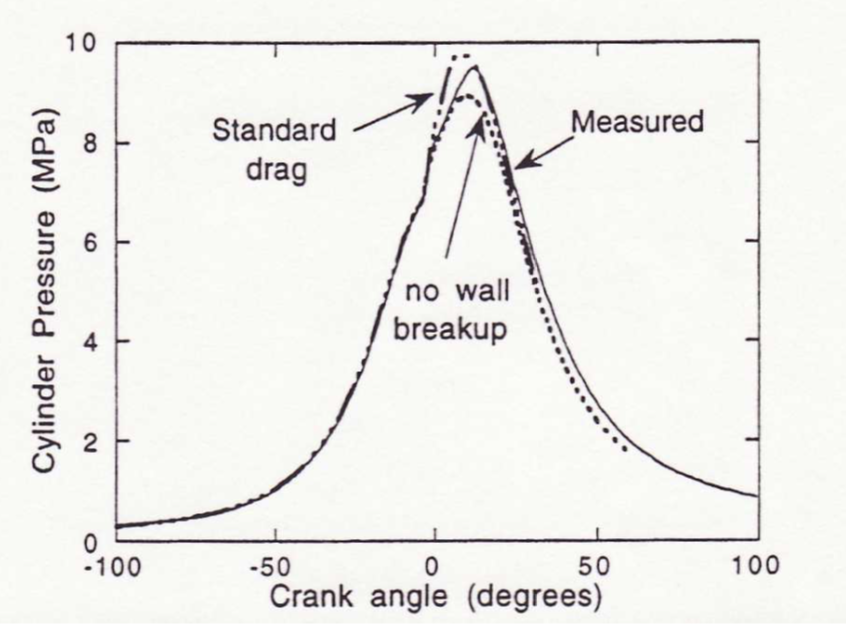
\includegraphics[width=0.5\textwidth]{figures/kiva3.png}
\end{figure}

Effects of drop drag and wall impingement on the combustion process.

\subsubsection{The spray model}

The spray model is a \textit{wave breakup model}, which take into account the wall impingement effects and drop drag varying coefficients. The fuel drop are injected with the size queal to the nozzle hole diameter and the number of drop is determined fromthe fuel flow rate. The mass of new droplets formed due to breakup is subtracted from the parent drop.\\
The high injection pressure in diesel engines produces a very high spray drop velocity with respect to the surrounfìding gas. Therefore the drop is subjected to high inertial forces which distort the drop into a disk shape. In order to model the trajectory of the drops, the drag coefficient must take into account this shape distortion since a distorted drop has a higher drag coefficient than a spherical drop.\\
Spray wall impingement is important since the impact of a drop on a heated surface may lead to its istantaneous vaporization or sliding and rebounding of a distorted drop (only the latter is modeled).

\subsubsection{The turbulence model}

The model is called \textit{RNG k-$\epsilon$}, an extra term is added to the dissipation equation which changes with the mean strain rate.
$k$ is the turbulent kinetic energy and $\epsilon$ is the dissipation rate:
\begin{equation}
    \frac{\partial \rho k}{\partial t}+\nabla\cdot(\rho u k)=...
\end{equation}
\begin{equation}
    \frac{\partial\rho\epsilon}{\partial t}+\nabla\cdot(\rho u \epsilon)=...
\end{equation}

\subsubsection{The ignition model}

A multistep kinetics model is adopted as the ignition model. The premise of the model is that \textit{degenerate branching} plays an important role in determining the cool flame and 2-stage ignition phenomena that are observed during the autoignition of hydrocarbon fuels.

\subsubsection{The combustion model}

This model is combind with the igniton model to simulate the overall combustion process in a diesel engine. The criterion to combine the ignition and combustion model is to switch between the models at $1000 K$. The igniton model is used when the temperature is lower than $1000 K$ to simulate the low temperature chemistry and viceversa. With this combustion model, the time rate of change of the partial density of species $m$ due to conversion from one chemical species to another, is given by:
\begin{equation}
    \frac{dY_{m}}{dt}=-\frac{Y_{m}-Y_{m}^{*}}{\tau_{c}}
\end{equation}
where $Y_{m}$ is the mass fraction of species $m$, $Y_{m}^{*}$ is the local equilibrium value of the mass fraction and $\tau_{c}$ is the characteristic time to achieve such equilibrium. An important aspect to this model is to formulate appropiately the characteristic time $\tau_{c}$ which is the sum of a laminar timescale and a turbulent timescale:
\begin{equation}
    \tau_{c}=\tau_{l}+f\tau_{t}
\end{equation}
where the \textit{delay coefficient $f$} determines the controlling role of turbulent effects.

\subsubsection{The emission model}

The extended \textit{Zel'dovich mechanism} is implemented to describe the $NO$ formartion. $NOx$ was found to be very sensitive to small changes in the computed gas temperature field. In order to obtain quantitative comparisons with experiments, a calibration factor $\beta$ is introduced:

\begin{equation}
    \bigg(\frac{dNO}{dt}\bigg)_{predicted}=\beta \bigg(\frac{dNO}{dt}\bigg)_{Zel'dovich}
\end{equation}

The soot emission model, written in the Arrhenius single step form, considers the rate of change of soot mass equal to the rate of formation less the rate of oxidation:

\begin{equation}
    \frac{dM_{soot}}{dt}= \frac{dM_{form}}{dt}- \frac{dM_{oxid}}{dt}
\end{equation}

\subsection{Spray generation}

Atomization is the process of conversion of the liquid fuel into small drops.\\ The aim is produce a high surface to mass ratio in the liquid phase in order to have a high evaporation rate. To this a high relative velocity between the liquid to be atomized and the sorrounding gas in needed which is what the \textit{pressure atomizers} and \textit{rotary atomizers} actually do. The \textit{airblast atomizers} instead eject a high velocity airstream on a slow liquid film. The Weber number provide a usel indication of both the quality and the nature of the atomization process.

\subsubsection{Spray characteristics}

\begin{itemize}
    \item \textit{Mean drop size}: the idea is to replace a given spray with one in which the droplets have the same diameter, retaining the characteristics of the original spray.
    \item \textit{Drop size distribution}: drop sizes range in diameter from $10$ to $400 \mu m$.
    \item  \textit{Patternation}: the uniformity of the circumferentual distribution of fuel in a conical spray. Poor patternation affects pollutants emission.
    \item \textit{Cone angle}: if the cone angle is narrow, drops are evenly dispersed through the entire spray (\textit{solid spray}). With swirl atomizers, a hollow conical structure of the spray is obtained allowing a better exposure to the sorrounding air.
    \item \textit{Dispersion}: the ratio of the volume of the spray to the volume of the fuel contained with it. A good dispersion allows a good mixing of the fuel with the surrounding gas, with an increase in the evaporation rate and heat release.
    \item \textit{Penetration}: maximum distance the spray reaches when injected in stagnant air. It is governed by the kinetic energy and the aerodynamic resistance. Compact narrow spray has high penetration. The penetration of a spray is greater than that of a single drop since the gas offers less resistance to the following drops which penetrate further.
\end{itemize}

\subsubsection{Simplex atomizer}

\begin{figure}[h!]
\centering
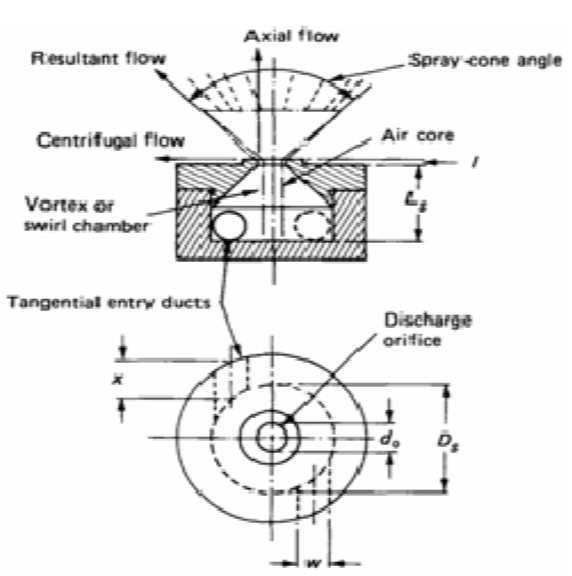
\includegraphics[width=0.5\textwidth]{figures/simplex.png}
\end{figure}

It is a pressure-swirl atomizer. The fuel is fed into a swirl chamber through tangential ports that give the fuel a high angular velocity. The rotating fluid flows through the orifice in the form of a hollo conical sheet. As the air pressure increases, the size distribution is shifted toward smaller drop diameters. The major drawback is that the flow rate varies as the square root of the pressure differential. Therefore, doubling the fuel flow rate requerise fourfold increase in pressure.

\subsubsection{Duplex atomizer}

The drawback of the simplex atomizer has led to the development of wide range atomizers such as \textit{duplex}, \textit{dual orifice} and \textit{spill} atomizers.\\

\begin{figure}[h!]
\centering
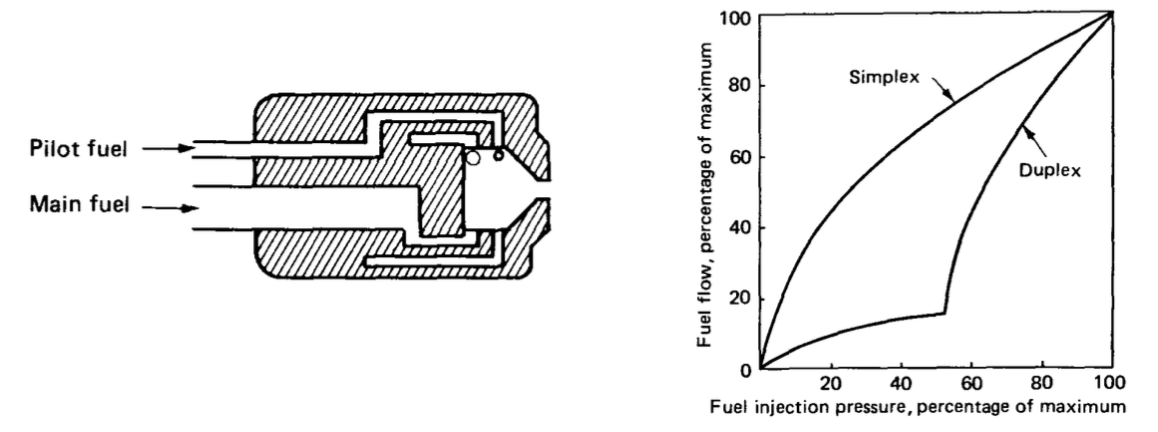
\includegraphics[width=0.8\textwidth]{figures/duplex.png}
\end{figure}

Two simplex nozzles are fitted concentrically, one inside the other. At low fuel flow all the fuel is supplied from the pilot nozzle, when the fuel pressure reaches a fixed value, the pressurising valve opens and admits fuel to the main nozzle.

\begin{figure}[h!]
\centering
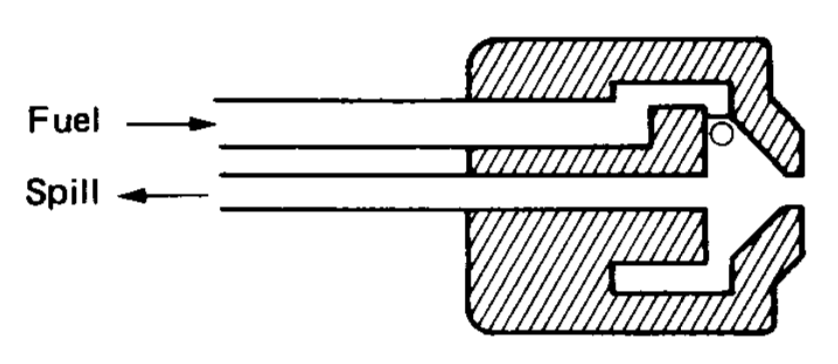
\includegraphics[width=0.5\textwidth]{figures/spill.png}
\end{figure}

The spill atomizer is a simplex atomizer but with a passage through which fuel can be spilled away from the atomizer. There is a constant use of a high pressure meaning that at low fuel flows the swirl is adequate to provide an efficient atomization of the fuel.
//In the rotary atomizer the fuel is fed into a rotating surface where it spreads out under the action of centrifugal force.

\begin{figure}[h!]
\centering
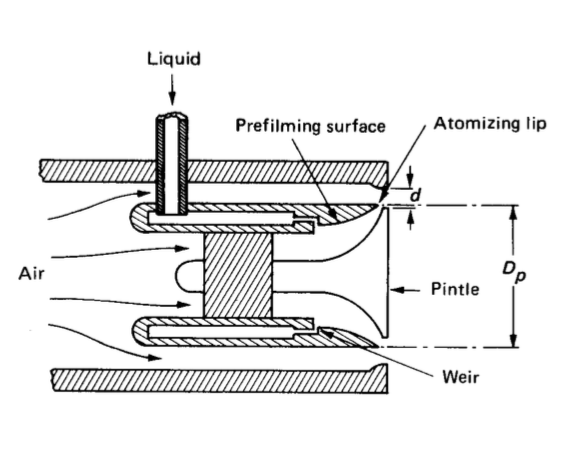
\includegraphics[width=0.5\textwidth]{figures/airblast.png}
\end{figure}

The airblast atomizer improve the atomization by prefilming the fuel and introducing air at high speed.

\newpage

\section{Reacting boundary layer}

TODO

\newpage

\section{Supersonic combustion and detonation}

In the study of detonation attention will be concentrated on the premixed flame. Reactions of the premixed gases are generally divided into three categories:

\begin{itemize}
    \item \textit{explosion}: the rate of heat generation is extremely fast, but it does not require the passage of a combustion wave through the exploding mixture
    \item \textit{deflagration}: the combustion wave propagates at subsonic speed
    \item \textit{detonation}: the combustion wave propagates at supersonic speed
\end{itemize}

Flames in combustibile gas mixture in tubes reaches enourmous velocities (~$3500 m/s$). Detonation waves are shock waves which are sustained by the energy of the chemical reaction that is initiated by the shock compression. Their rate of propagation is limited by the rate at which a shock wave can travel.

\subsection{Shock wave in a neutral gas}

Consider a long tube closed at the left by a piston. A small velocity $dw$ is imparted to the piston, this movement produces in the gas a weak compression wave that travels from left to roght with the velocity of sound. The gas to the right of the wave front is at rest, while the gas between the wave front and the piston is compressed adiabatically by $dp$ and has the velocity $dw$. Then, the velocity of the piston is increased by another $dw$, a second compression wave is produced in the gas. By ripetition of this procedure the velocity of the piston is brought to the final velocity $w$.

\begin{figure}[h!]
\centering
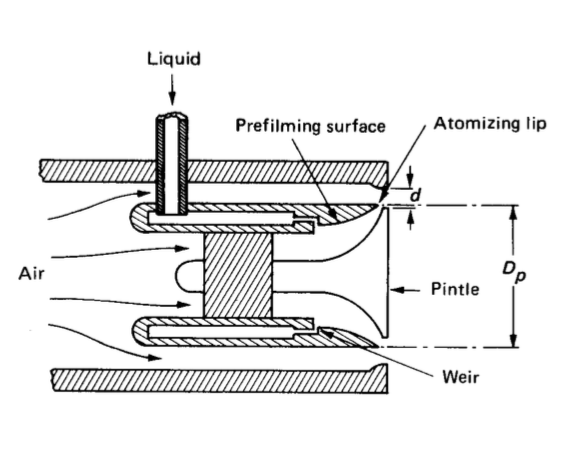
\includegraphics[width=0.5\textwidth]{figures/airblast.png}
\end{figure}

A step-like set of waves is produced. The upper steps of the terrace have greater velocity than the lower steps since the temperature and theredore the velocity of sound is larger in the gas in the upper steps. As soon as the steps are merged, a shock wave with very high steep pressure gradient is formed. After the piston has attained its constant velocity $w$, the column of gas is pushed ahead at the same velocity $w$. Work must constantly be performed by the piston in order to mantain the motion.\\
Consider a coordinate system moving with the wave front. Since the process is stationary, the masses, momenta and energies are constant:

\begin{equation}
    \frac{u_{1}}{v_{1}} =  \frac{u_{2}}{v_{2}}
\end{equation}

\begin{equation}
    \frac{u_{1}_{2}}{v_{1}} + p_{1} =  \frac{u_{2}^{2}}{v_{2}} + p_{2}
\end{equation}

\begin{equation}
    E_{1} + \frac{u_{1}_{2}}{2} + p_{1}v_{1} = E_{2} + \frac{u_{2}_{2}}{2} + p_{2}v_{2}
\end{equation}

The equations represent the conservation of mass, momentum and energy.\\
The velocity of propagation $D$ of the shock wave into the gas at rest is found to be:

\begin{equation}
    D = u_{1} = v_{1}\sqrt{\frac{p_{2}-p_{1}}{v_{1}-v_{2}}}
\end{equation}


















\end{document}

